% ********** Readout Chapter **********
\chapter{Detector Readout}
\label{cha:readout}
\epigraph{``The audience is the most revered member of the theater. Without an audience there is no theater.''}{\epiauthor Viola Spolin}
\section{Introduction}
\label{sec:readout-introduction}

Like all high-sensitivity detectors operating in the far-infrared, cold-electron bolometers need to be readout using amplification \parencite{Rieke2007}. This amplification is of either the voltage or the current, with the quantity not being amplified for readout usually providing the bias. \textcite{Golubev2001} provide a good discussion of the advantages and disadvantages of current-bias versus voltage-bias for use with \glspl{acr:CEB}, along with a basic schematic for each case.
\par 
In reality, the \glspl{acr:SQUID} and their associated electronics used to amplify current in a voltage bias regime are both more expensive and more complex to set up compared to the voltage amplifiers used for current biased measurements. This means that it is often preferable to use a current biased system for early device development.
\par 
During the development of \glspl{acr:SiCEB} described in this work, numerous iterations of voltage amplifier have been used. Each readout system was designed to offer the possibility of improved device characterisation, from either a lower contribution to the noise measurement or by allowing measurements to higher frequencies of readout.
\par
In addition to changes that were required to the amplification system, it has also been necessary to change the exact technique by which the detector has been biased. The main driver for these changes has been the desire to reduce electrical noise input to the device, as well as to create the most stable and capable testing regime possible.

\section{Requirements of the Readout System}\label{ssec:readout_requirements}
In order to specify a readout system, it is important to define a number of desirable goals for its performance. For the early development stage testing of \glspl{acr:CEB} the following desired points were set:
\begin{itemize}
\item The system had to be as simple as possible. This is to say that the design and operation of the readout should not become a distraction from the testing of devices.
\item The system needed to contribute a sufficiently low electrical noise that noise measurements of the detector could be successfully  performed.
\item The system was capable of measuring the speed of response of the detector by measurement of the roll-off of device noise.
\end{itemize}
Although it was possible to estimate both the speed and expected noise levels for a \gls{acr:CEB}, these estimates were only vague `ball-park' figures. This meant that it was necessary to produce a testing system believed to be capable of meeting these criteria and then to make improvements as required. Further to these requirements, any system needed to be able to perform DC-measurements, such as recording \gls{acr:IV} curves with a high degree of stability.

\section{Initial Testing System}
\label{sec:initial_readout_system}
\subsection{Initial Readout System}
\label{ssec:readout-prelim}
\begin{figure}[ht]
\begin{center}
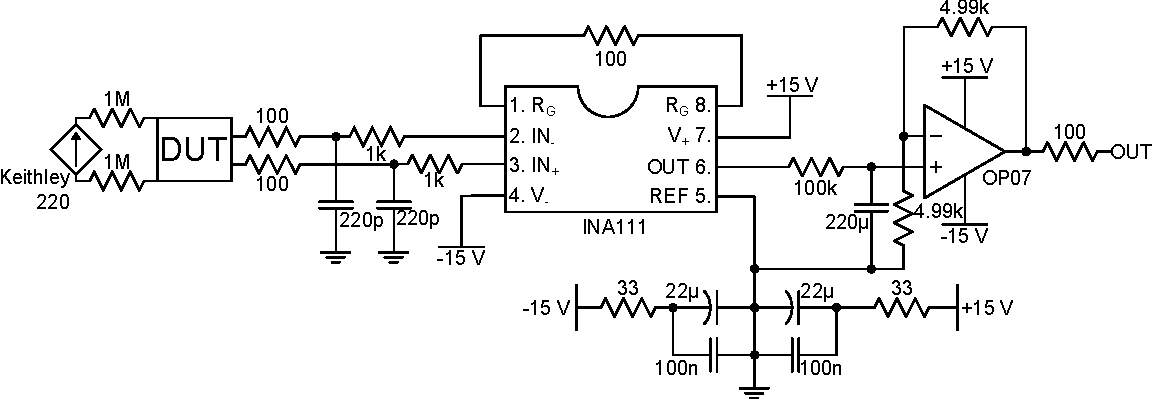
\includegraphics[width = 0.95\textwidth]{figures/RTD_amp.pdf}
\caption[Initial readout system using RTD amplifier and programmable current source]{Initial bias and readout system using a Keithley 220 Programmable Current Source to bias the device under test (DUT). The voltage is then amplified by the INA111 differential amplifier (configured for a gain factor of 500) and then by the OP07 operational-amplifier (configured to give a gain of two).}
\label{fig:rtd_readout_amp}
\end{center}
\end{figure}
The initial amplification system used was heavily based upon an existing circuit designed to readout \glspl{acr:RTD}. This was used as it was readily available within the department and early (somewhat optimistic) estimations of device performance indicated that noise measurements would be possible. This amplifier was used in conjunction with a Keithly 220 Programmable Current Source to provide the bias across the device. Figure~\ref{fig:rtd_readout_amp} shows the circuit diagram of the amplifier used here, along with the connection to the current source. To perform an \gls{acr:IV} measurement, the current source, which is controlled by a computer, is stepped through the desired range of values and at each step a \gls{acr:DAQ} records the amplified voltage across the device.
\par 
The \textcite{INA1112010} and \textcite{OP07DS} state that both these amplifiers have, when operating in the configuration shown in Figure~\ref{fig:rtd_readout_amp}, a noise voltage, referred to the input, of $10~\mathrm{nV\,Hz}^{-\nicefrac{1}{2}}$. In order to understand how the internal noise of these amplifiers contributes to the total noise measured at the output of the system, we can think of each of the two amplifiers as containing some source which generates a noise voltage with a spectral density of $e_{\mathrm{n}}$ and a \textit{black-box} which provides the gain while generating no noise. This is illustrated in Figure~\ref{fig:series_amp_model}.
\begin{figure}[ht]
\begin{center}
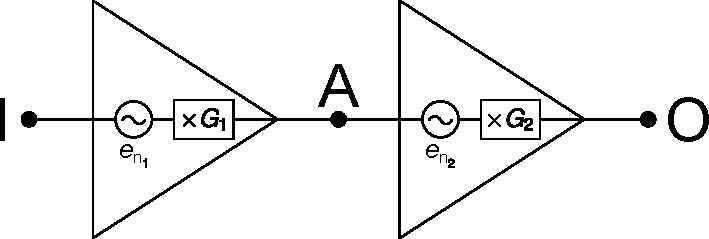
\includegraphics[width = 0.95\textwidth]{figures/amp_noise_model.pdf}
\caption[Noise model of series amplifiers]{Simple model of two amplifiers working in series. Each amplifier contains a component which generates a noise voltage with spectral density $e_{\mathrm{n}}$ before an ideal, noiseless, component amplifies the signal by a gain factor of $G$.}
\label{fig:series_amp_model}
\end{center}
\end{figure}
\par 
In Figure~\ref{fig:series_amp_model}, we see that if there is no input signal at point I then the input to the second amplifier, point A, will consist of only the noise generated in the first amplifier, multiplied by that amplifier's gain factor. The uncorrelated noise from the second amplifier is then added to the amplified noise from the first and both are multiplied by the gain of the second amplifier. From this, we can define the total noise, $e_{\mathrm{tot}}$, at the output of this system, in the absence of any input signal, as:
\begin{align}
e_{\mathrm{tot}} &= \sqrt{\left(e_{\mathrm{n_{1}}} \times G_{1}\right)^{2} + e_{\mathrm{n_{2}}}^{2}} \times G_{2}\, . \label{eqn:total_series_amp_noise}\\
\intertext{If, as is the case in Figure~\ref{fig:rtd_readout_amp}, $e_{\mathrm{n_{1}}} \times G_{1} \gg e_{\mathrm{n_{2}}}$ then we can say:}
e_{\mathrm{tot}} &\approx e_{\mathrm{n_{1}}} G_{1} G_{2}\, . \label{eqn:approx__series_amp_noise} \\
\intertext{We can define the input referred noise voltage spectral density, $e_{\mathrm{RTI}}$, simply as:}
e_{\mathrm{RTI}} &= \frac{e_{\mathrm{tot}}}{G_{\mathrm{tot}}}\, , \label{eqn:noise_RTI} \\
\intertext{where $G_{\mathrm{tot}}$ is the product of the various gain stages, given by:}
G_{\mathrm{tot}} &= \prod_{n} G_{n}\, . \label{eqn:total_gain}
\end{align}
\par 
By applying Equation~\ref{eqn:total_series_amp_noise} for the system shown in Figure~\ref{fig:rtd_readout_amp} ($e_{\mathrm{n_{1}}} = e_{\mathrm{n_{2}}} = 10~\mathrm{nV\,Hz}^{-\nicefrac{1}{2}}$, $G_{1} = 500$ and $G_{2} = 2$), we find that $e_{\mathrm{RTI}} = 10.00002~\mathrm{nV\,Hz}^{-\nicefrac{1}{2}}$. The above approximation can be verified by calculating $e_{\mathrm{RTI}}$ again using Equation~\ref{eqn:approx__series_amp_noise}, this gives $e_{\mathrm{RTI}} \approx 10~\mathrm{nV\,Hz}^{-\nicefrac{1}{2}}$\label{res:RTD_amp_noise}. This shows that, in this case, the internal noise from the second amplifier is contributing only $0.0002~\%$ of the  noise at the output.
\par 
It is possible to characterise an amplifier by measuring three simple parameters of the amplifier: gain, bandwidth and internal noise. The gain can be found by measuring how much a signal (a simple sinusoidal wave for example) is amplified; the bandwidth of the amplifier can be found by measuring the frequency at which the noise spectral density decreases from $e_{\mathrm{tot}}G_{\mathrm{tot}}$ (this can also serve as a measure of the uniformity of the gain across a wide range of frequencies); finally, the internal noise (referred to the amplifier's input) can found be from the noise spectral density, corrected for the measured gain, when the input of the amplifier is shorted (no input signal).
\par
\begin{figure}[t]
\begin{center}
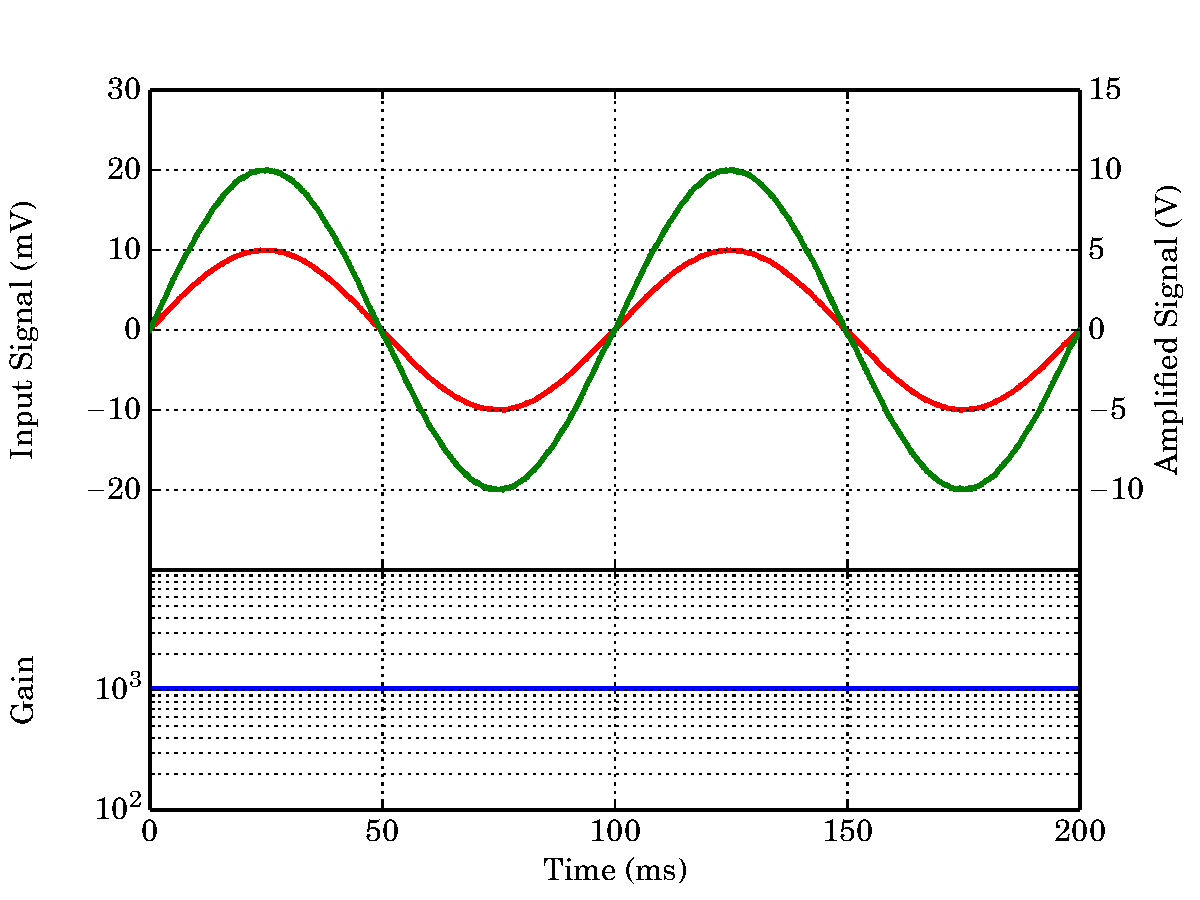
\includegraphics[width = 0.95\textwidth]{figures/RTD_amp_gain}
\caption[Gain measurement of original amplifier]{Gain measurement of RTD amplifier using a $10~\mathrm{Hz}$ sinusoidal wave. Upper plot---Input signal (red, primary vertical axis) compared to the amplified signal (green, secondary vertical axis). Lower plot---Gain measured from taking the ratio of the amplified and input signals.}
\label{fig:RTD_amp_gain}
\end{center}
\end{figure}
Figure~\ref{fig:RTD_amp_gain} shows the amplification of a $10~\mathrm{Hz}$ sinusoidal wave generated by a signal generator, the output of which was split between the amplifier to be tested and a direct input to a digital oscilloscope. The input signal (red, shown on the primary vertical axis of the upper plot of Figure~\ref{fig:RTD_amp_gain}) was measured to have a peak amplitude of $10~\mathrm{mV}~\left(V_{\mathrm{rms}} = 7.07~\mathrm{mV}\right)$. The amplified signal (green, secondary vertical scale) was measured as having a peak amplitude of $10~\mathrm{V}~\left(V_{\mathrm{rms}} = 7.07~\mathrm{V}\right)$, from this, it is clear that the gain factor of the amplifier is $1000$ at the voltage peaks. The uniformity of the gain, for various input amplitudes, was verified by simply taking the ratio of these two signals at all points; the result of this is shown in the lower plot of Figure~\ref{fig:RTD_amp_gain}. It can clearly be seen that the gain factor of $1000$ does not vary with the amplitude of the input signal (up to $10~\mathrm{V}$). The \textcite{INA1112010} states that the input amplitude range (the range over which the input is amplified by a constant gain) of this device is $12.7~\mathrm{mV}$ when operating at a gain of $1000$.
\par 
The next stage in characterising this amplifier was to measure the bandwidth, in frequency, over which a signal is consistently amplified. This was performed by using a signal generator to output a white noise signal\footnote{The \textcite{AG33220ADS} states that this device has a bandwidth, when generating noise, of $9~\mathrm{MHz}$.} of known amplitude. Similarly to the previous test, this signal was then split, with one output being passed directly to a digital oscilloscope and the other being amplified before being passed to the oscilloscope. The digital oscilloscope was also used to process both of these signals by computing the \gls{acr:FFT} of both. When defining the frequency bandwidth of an electronic device, it is usual to take the frequency that the voltage throughput has fallen to a factor of the square root of two times the maximum throughput. This is called the 3-dB bandwidth, since:
\begin{align}
20\log_{10}\left(\frac{1}{\sqrt{2}}\right) &\approx -3~\mathrm{dB}\, . \label{eqn:3dBV}
\intertext{More correctly, the 3-dB bandwidth is defined as the frequency at which the power throughput has fallen by a factor of one half, i.e.:}
10\log_{10}\left(\frac{1}{2}\right) &\approx -3~\mathrm{dB}\, . \label{eqn:3dBP}
\end{align}
\begin{figure}[t]
\begin{center}
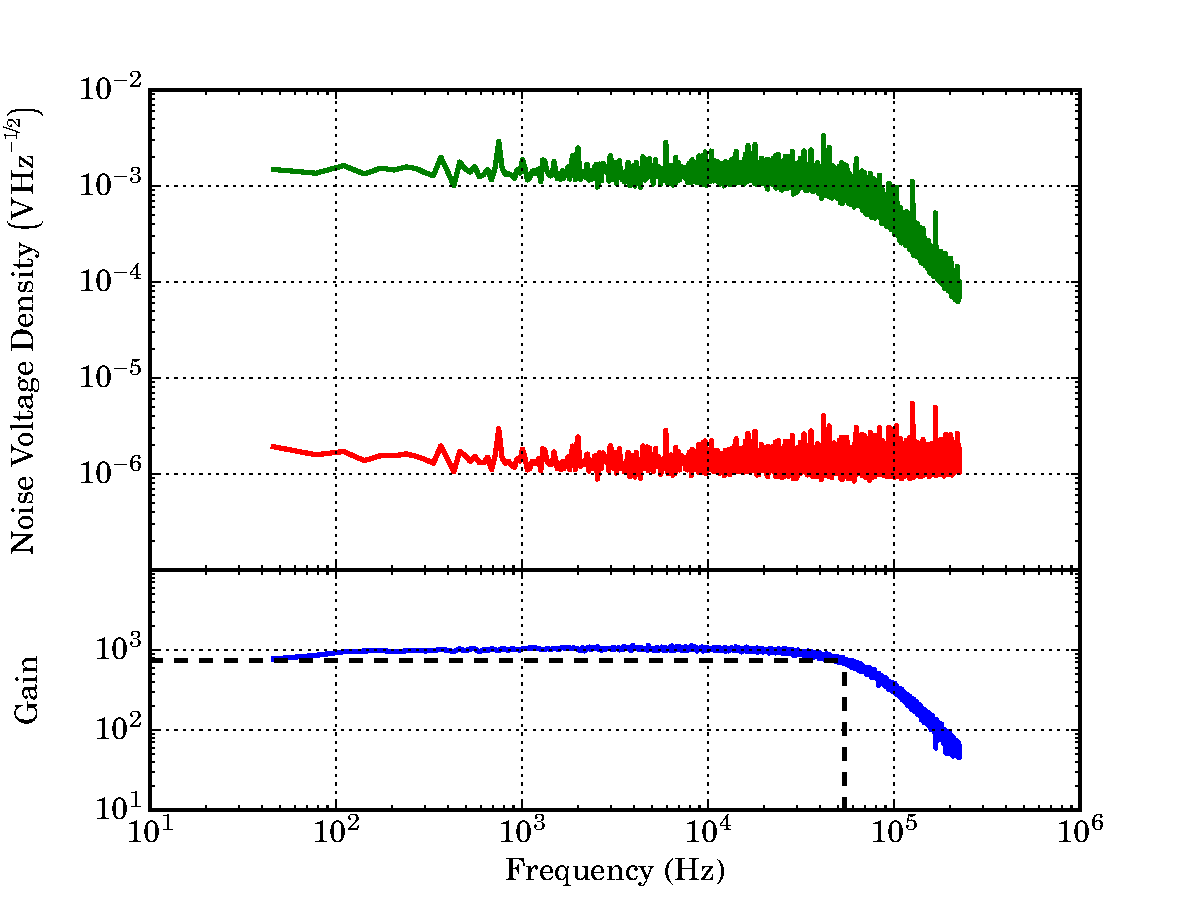
\includegraphics[width = 0.95\textwidth]{figures/RTD_amp_BW}
\caption[Bandwidth measurement of original amplifier]{Bandwidth measurement of RTD amplifier. A white noise signal was generated by a signal generator, this was split with one feed being fed directly to the oscilloscope (red line) and one feed being amplified first (green line). The ratio (the gain of the amplifier) is shown on the lower plot the $3~\mathrm{dB}$ level and corresponding frequency limit to the bandwidth are shown by the dashed line in the lower plot.}
\label{fig:RTD_amp_BW}
\end{center}
\end{figure}
\par 
Figure~\ref{fig:RTD_amp_BW} shows the result of the bandwidth measurement. It is clear from the figure that, at frequencies below $10~\mathrm{kHz}$, the output of the amplifier (green trace on upper plot) differed only from the generated noise (red trace on upper plot) by the gain factor of $1000$. As the frequency increased the gain factor (blue trace on lower plot) ceased to be constant and started to decrease. Using Equation~\ref{eqn:3dBV}, the 3-dB bandwidth corresponds to the gain dropping to $731$; this occurred at a frequency of $55~\mathrm{kHz}$\label{res:RTD_amp_BW}, which is illustrated by the dashed line on the lower plot of Figure~\ref{fig:RTD_amp_BW}.
\par 
The final part of characterising the amplifier was to measure the input-referred noise. As seen earlier in this section for the configuration of this amplifier (shown in Figure~\ref{fig:rtd_readout_amp}) the expected input referred noise was $10~\mathrm{nV\,Hz}^{-\nicefrac{1}{2}}$ (explained on Page~\pageref{res:RTD_amp_noise}). To measure this quantity, the input of the amplifier was shorted and the output of the amplifier was measured as in the previous tests.
\begin{figure}[t]
\begin{center}
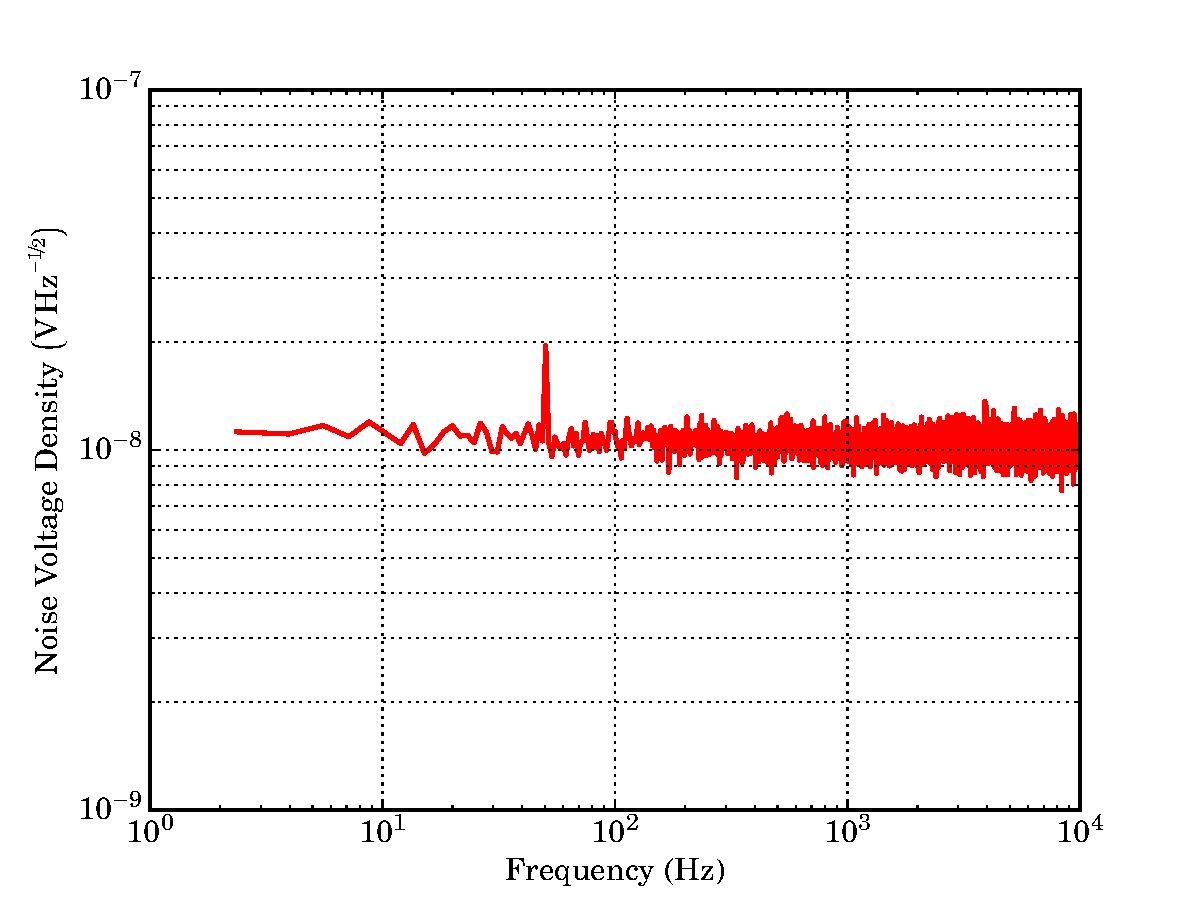
\includegraphics[width = 0.95\textwidth]{figures/RTD_amp_IRN}
\caption[Input referred noise of original amplifier]{Measurement of the internal noise of the original amplifier, referred to the input of the amplifier. The measurement was performed by shorting the input of the amplifier and measuring the output of the amplifier with a digital oscilloscope, which also computed the \gls{acr:FFT}.}
\label{fig:RTD_amp_IRN}
\end{center}
\end{figure}
\par 
Figure~\ref{fig:RTD_amp_IRN} shows the measured noise spectrum for the amplifier (as referred to the input), measured up to $10~\mathrm{kHz}$. From this figure, we can see that the internal noise is equivalent to a noise source of $10~\mathrm{nV\,Hz}^{-\nicefrac{1}{2}}$ at the input of the amplifier. This is the value which was predicted on Page~\pageref{res:RTD_amp_noise} and this result, along with the results of the other tests carried out thus far, indicated that the amplifier system was performing as designed.

\subsection{Initial Bias System}
\label{ssec:bias_prelim} 
The amplifier only contributes one part of the total performance of the electronic system. The source of biasing current also plays a substantial role in the final performance. Unlike the amplifier, the speed or bandwidth of this current source is not of high importance since the \gls{acr:IV} measurements can performed at a low frequency and noise measurements are measured with the device at a constant (DC) bias. The bias circuitry can, however, have a negative effect on measurement by either failing to provide a stable bias and thus causing some degree of \textit{jitter} in a measurement or by adding undesired levels of noise (either as white noise or as finite tones). In the case of the current supply contributing additional noise, this could, in turn, cause additional energy to be dissipated across the device being tested and thus affect the result.
\par 
In the first system used, the current bias was provided by a Keithley 220 Programmable Current Source; this unit is capable of providing currents between $500~\mathrm{fA}$ and $100~\mathrm{mA}$ with a peak-to-peak noise level of between $400~\mathrm{ppm}$ and $100~\mathrm{ppm}$ depending on the output range specified\footnote{The full specifications of Keithley's 220 current source are stated in the \textcite{Keithley220DS}.}.
\par 
In order to test the effect of the current source, two simple measurements were performed using a \textit{dummy} device (typically a resistor with an appropriate value) as the DUT in Figure~\ref{fig:rtd_readout_amp}\footnote{The $1~\mathrm{M\Omega}$ resistors shown in Figure~\ref{fig:rtd_readout_amp} were used offer protection to sensitive detectors and were not included in this test.}. Firstly, a test was carried out to ensure that the output of the device was stable enough to allow for reliable measurements. This was performed in two parts: initially the Keithley 220 current source was set to a constant value (specifically $10~\mathrm{\upmu A}$) and the voltage across the \textit{dummy} device (a $1~\mathrm{k\Omega}$ resistor) was measured multiple times using a reliable \gls{acr:DAQ}; after this the current across the resistor was increased in steps through a defined range and the voltage across the DUT was measured for each step. These tests were selected as they closely resemble the tests which were to be performed on the eventual \gls{acr:SiCEB} devices.
\begin{figure}[t]
\begin{center}
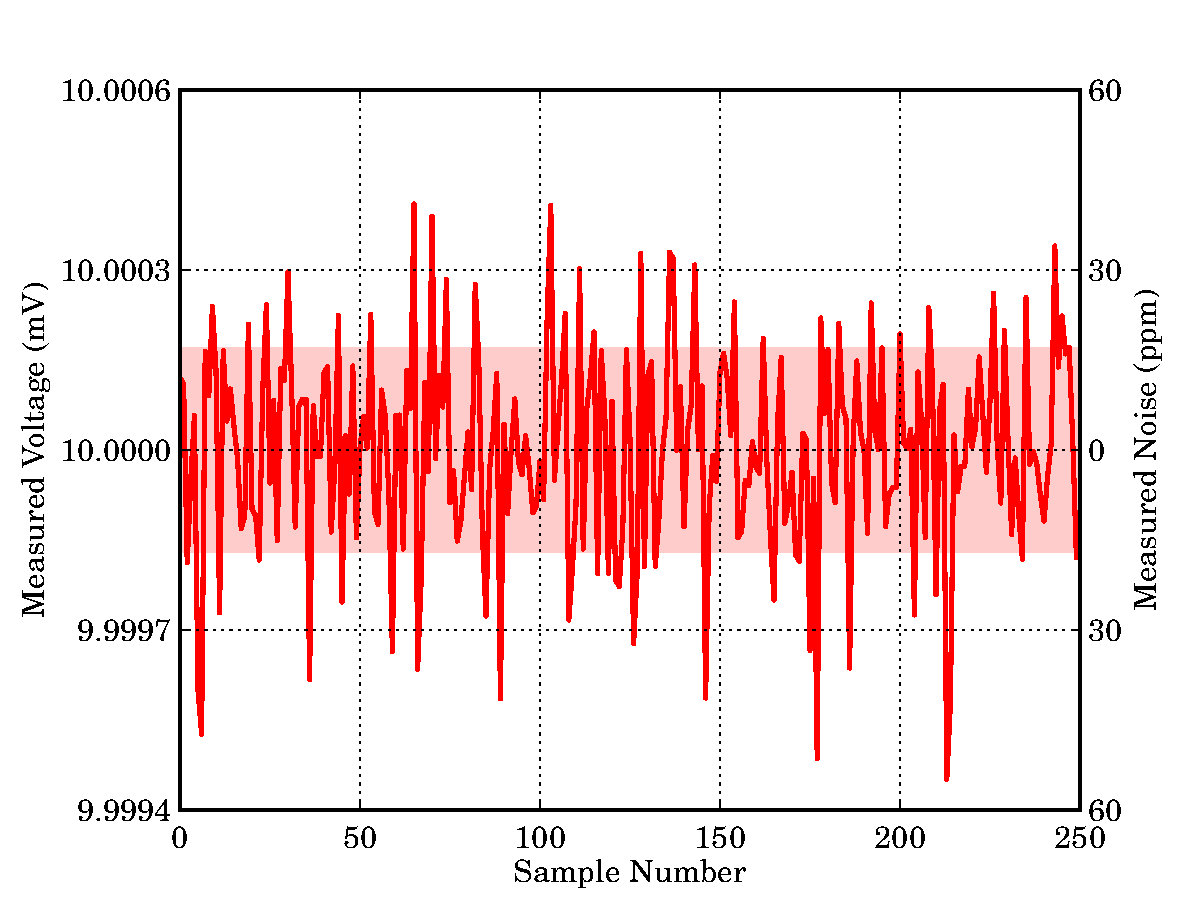
\includegraphics[width = 0.95\textwidth]{figures/keithley220_jitter}
\caption[Jitter from a Keithley 220 Current Source]{Jitter in a measurement caused by current supplied by a Keithley 220 Programmable Current Source. The current source was set to output a constant current of $10~\mathrm{\upmu A}$ which was driven across a $10~\mathrm{k\Omega}$ resistor. Multiple measurements were made with a trusted data acquisition system. The primary vertical axis shows the voltage measured across the resistor in each measurement (the expected voltage was $10~\mathrm{mV}$); the secondary vertical axis shows the jitter or noise about the expected value in terms of noise parts per million; the shaded region shows the standard deviation of the noise about the expected value.}
\label{fig:Keithley220_jitter}
\end{center}
\end{figure}
\par 
Figure~\ref{fig:Keithley220_jitter} shows the measured jitter of a signal caused by the Keithley 200 unit. The signal varied around the expected value of $10~\mathrm{mV}$ by up to $550\mathrm{nV}$. The signal was measured by a trusted data acquisition system using shielded cables. This variation is equivalent to a peak-to-peak noise level of $110~\mathrm{ppm}$. The \textcite{Keithley220DS} states that when outputting a current of $10~\mathrm{\upmu A}$ the expected peak-to-peak noise level is $100~\mathrm{ppm}$; although this is slightly lower than the measured value and thus indicates either an additional noise source or an issue with the unit, the measured jitter was still sufficiently low for preliminary measurements. 
\par 
There are several possible reasons for the small amount of additional jitter measured in this test. Both the Keithley 220 unit used and the triaxial cables used as interconnects between the current source and the device under test were several years old and it is entirely possible that a number of small breaks were present in either the cable's inner guard layer or the insulator; this could cause current to be lost between the innermost conductor and the outermost shield layer and thus, for current to be lost between these two. The age of the unit may also have meant that some of the internal components had degraded and were no longer working within their original specification. It is most likely that a combination of these factors caused the additional noise measured. It is also possible that the degrading of the interconnecting cables could have made the system more susceptible to electromagnetic pickup.
\begin{figure}[t]
\begin{center}
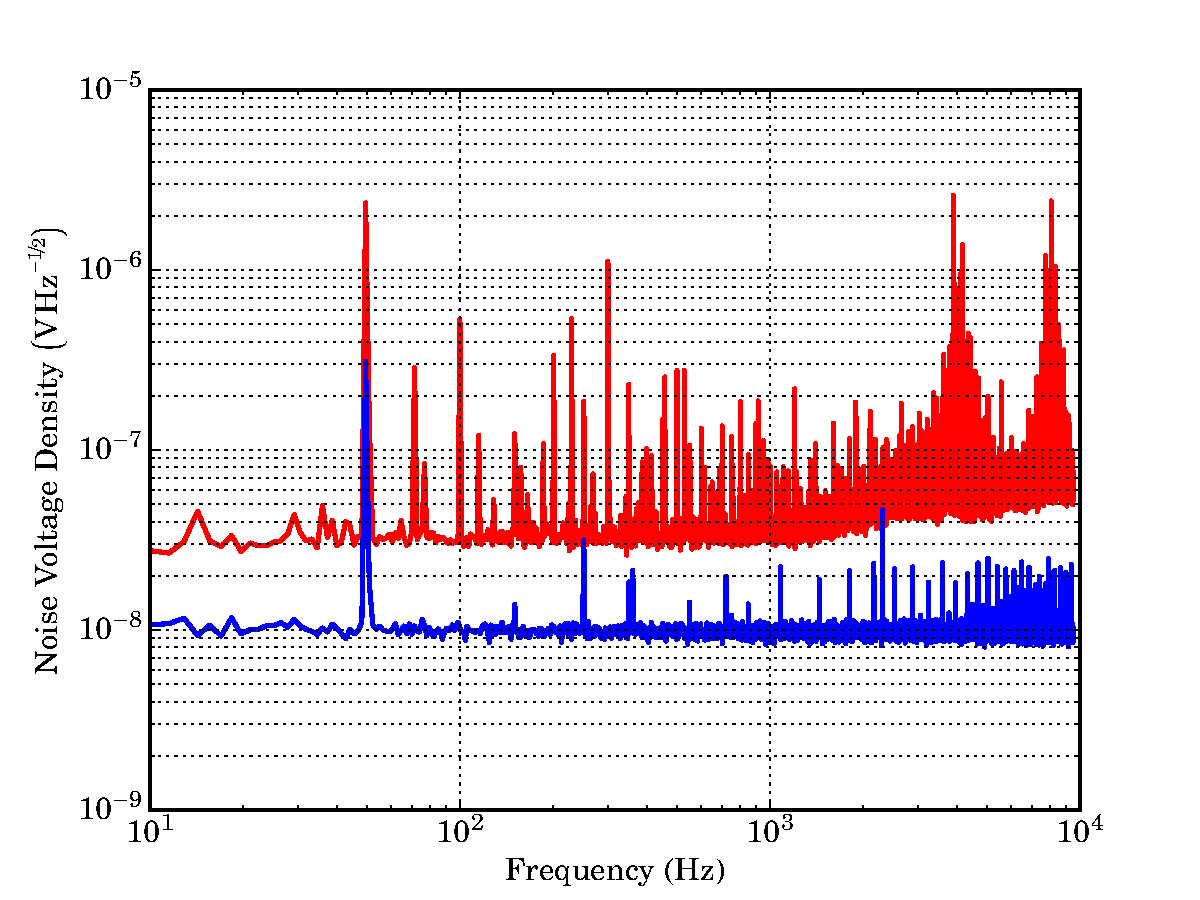
\includegraphics[width = 0.95\textwidth]{figures/keithley220_noise}
\caption[Noise spectrum from a Keithley 220 Current Source]{Noise spectrum measured across a resistor which was biased by the Keithley 220 Current Supply. A current of $10~\mathrm{\upmu A}$ was driven across the resistor and the voltage (and noise spectrum) was measured using a digital oscilloscope. It was expected that the noise spectrum would be dominated by the amplifier noise of $10~\mathrm{nV\,Hz}^{-\nicefrac{1}{2}}$; it is clear that this measurement shows a white noise level greater than this and is dominated by several other sources.}
\label{fig:Keithley220_noise}
\end{center}
\end{figure}
\par
The noise voltage spectrum measured across the resistor is shown in Figure~\ref{fig:Keithley220_noise}; this did not resemble the \textit{clean} spectrum seen in Figure~\ref{fig:RTD_amp_IRN}, instead there was a substantial tone, due to mains pickup, seen at $50~\mathrm{Hz}$. Along with several harmonics of this tone, there were various other noise sources evident, including two large clusters of tones at $4$ \& $8~\mathrm{kHz}$. These large clusters of noise tones were of particular concern, as they indicated that in addition to the desired DC biasing signal, there could have been a substantial amount of power dissipated in the device under test from these sources. The cause of this noise was confirmed by repeating the measurement across the resistor having disconnected the current supply. The result of this closely resembled that shown in Figure~\ref{fig:RTD_amp_IRN} and showed that the noise was due to the presence of the current supply. By disconnecting the interconnecting triaxial cable from the current supply, while leaving it attached to the device under test, it was found that the two clusters of high frequency tones were no longer present, this indicated that these were due to internal components within the current supply unit. However, many of the lower frequency tones remained, these were attributed to electromagnetic pickup in the cable. This result meant that the Keithley 220 current supply would not be appropriate for use when carrying out noise measurement, since there was sustaintial contamination of the signal.

\section{Revisions to the Initial Bias System} \label{sec:RTD_bias}
\subsection{Changes Made and Advantages} \label{ssec:RTD_bias_changes&advantages}
As was found by the test described in the previous section, the Keithley 220 current source was not appropriate for noise measurement, since there was substantial contamination (at AC frequencies) of the biasing signal from both electromagnetic pickup and the issues within the unit itself. To address this, a simple circuit was constructed which generated a controlled differential signal, which had an amplitude determined by a controllable input signal. This signal could then be converted to a biasing current via a pair of resistors and the resulting current was found using Ohm's Law and measuring the voltage dropped across these biasing resistors.
\begin{figure}[t]
\begin{center}
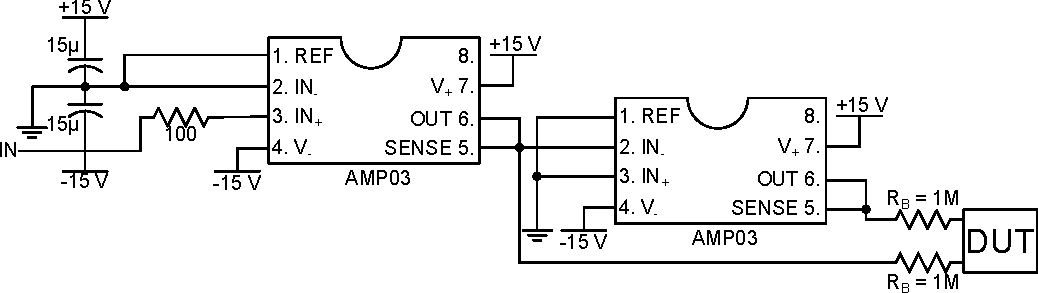
\includegraphics[width = 0.95\textwidth]{figures/RTD_bias}
\caption[Internal bias generator used with initial amplifier]{Circuit diagram for the custom-made internal bias generator used with the first amplifier. A single ended input was fed to the non-inverting input of a unity gain amplifier, the output of this amplifier was split with one feed being supplied to the inverting input of a second unity gain amplifier. The output of this amplifier, along with that of the first, was then used to bias the device under test via a pair of biasing resistors.}
\label{fig:RTD_bias}
\end{center}
\end{figure}
\par 
There are several advantages to housing the biasing unit inside the casing of the amplifier, which during device testing was directly mounted to a cryostat. Firstly, since no interconnecting cabling was required, the possibility of electromagnetic pickup was greatly reduced. Secondly, due to the close physical proximity of the amplifier and the current supply, it was possible to have greater control over the grounding of these two components and thus remove any ground loops which could have offset a measurement or contributed to the total noise measured. Further to this, since the biasing signal was now sent using a differential connection, there was no connection to ground across the device under test is fully isolated from any possible ground loops or other contamination from the ground line. Finally, since the amplitude of the current was not directly controlled by the bias generator but instead was governed by an external source, it was possible to produce a smooth range of currents, as opposed to the Keithley unit which was only able to step current, albeit in relatively small steps.
\par 
The bias generator worked by using two unity gain amplifiers to generate a differential biasing signal, $V_{\mathrm{in}}$, from a single-ended input. The input was fed into the non-inverting input of the first amplifier, the output of this was equal in amplitude to the input signal and  was then split, with one feed connected to the inverting input of the second amplifier. The output of the second amplifier was again equal in amplitude to the input signal but had the opposite sign; the output of this amplifier, along with that of first amplifier, served as the biasing voltage. This biasing voltage, $V_{\mathrm{bias}}$, formed a differential signal and was given by:
\begin{align}
V_{\mathrm{bias}} &= V_{+} - V_{-}, \label{eqn:diffBiasGen}
\intertext{where $V_{+}$ and $V_{-}$ are the outputs of the first and second amplifiers respectively. Since, in this case, the outputs of these amplifiers were $V_{+} = +V_{\mathrm{in}}$ and $V_{-} = -V_{\mathrm{in}}$, the final biasing voltage was given by:}
V_{\mathrm{bias}} &= 2 V_{\mathrm{in}}. \label{res:RTDVbias}
\intertext{The biasing current, $I_{\mathrm{bias}}$, across the device under test is the same as the current through the two biasing resistors, which from Ohm's Law is given by:}
I_{\mathrm{bias}} &= \frac{V_{\mathrm{R}}}{2 R_{\mathrm{bias}}}, \label{eqn:OhmsRbias}
\intertext{where $V_{\mathrm{R}}$ is the voltage dropped across the two biasing resistors. By measuring the voltage across the device under test, $V_{\mathrm{DUT}}$, and knowing the voltage generated by the bias circuitry, the voltage dropped across the biasing resistor was given by:}
V_{\mathrm{R}} &= V_{\mathrm{bias}} - V_{\mathrm{DUT}}. \label{eqn:RbiasVgeneric}
\intertext{By using the result of Equation~\ref{res:RTDVbias}, the above can be written as:}
V_{\mathrm{R}} &= 2 V_{\mathrm{in}} - V_{\mathrm{DUT}}. \label{eqn:RbiasVRTD}
\intertext{Finally, combining this with Equation~\ref{eqn:OhmsRbias}, the biasing current can be calculated by:}
I_{\mathrm{bias}} &= \frac{2 V_{\mathrm{in}} - V_{\mathrm{DUT}}}{2 R_{\mathrm{bias}}}. \label{res:RTDIbias}
\end{align}
\par 
\begin{figure}[t]
\begin{center}
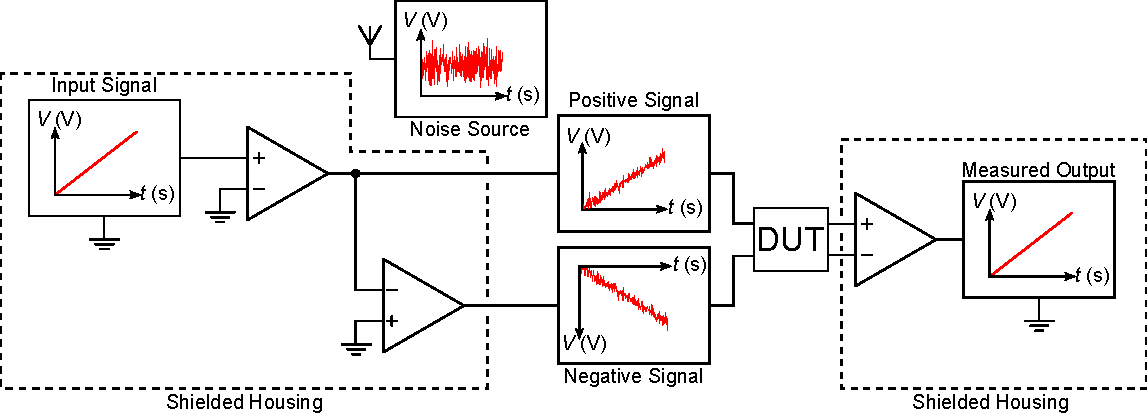
\includegraphics[width = 0.95\textwidth]{figures/differential_noise}
\caption[Rejection of common-mode noise in a differential bias and readout system]{Rejection of common-mode noise in a differential-signal bias and readout system. The two amplifiers which make up the differential signal generator produce two signals, which are equal and opposite to each other and related in magnitude to the input signal. This is then carried, by a pair of wires, through an unshielded environment. Any electromagnetic pickup adds to both of these signals as a common mode; this does not affect the difference in amplitude between the two signals and thus is not measured by the final differential amplifier.}
\label{fig:differential_noise_rejection}
\end{center}
\end{figure}
There were further advantages of this biasing regime, offered by the fact that the system now used a differential signal to bias the device under test, since the device under test was now isolated from the ground line, which is often a source of signal contamination. This regime also offers a dramatic reduction in the effect of electromagnetic pickup. As this differential bias generator produced two signals of equal and opposite voltage and since noise due to electromagnetic pickup would have added to both, this meant that the difference between the two signals, at any given time, remained the same and the output of the final amplifier, which only depended on this difference, was not affected. In terms of differential signals, a change which maintains the same difference between the two signals is referred to as a common mode and when the difference between the two is affected, there is said to be a normal mode. This concept is illustrated in Figure~\ref{fig:differential_noise_rejection}.

\subsection{Performance of the Updated Bias System}
\label{ssec:RTD_bias_performance} 
In order to ascertain whether or not this current generator offered improved performance over the Keithley 220, the same tests that were described in Section~\ref{ssec:bias_prelim} were repeated with the new system. Of particular interest were the results of measuring the noise spectrum produced by this system.

\begin{figure}[t]
\begin{center}
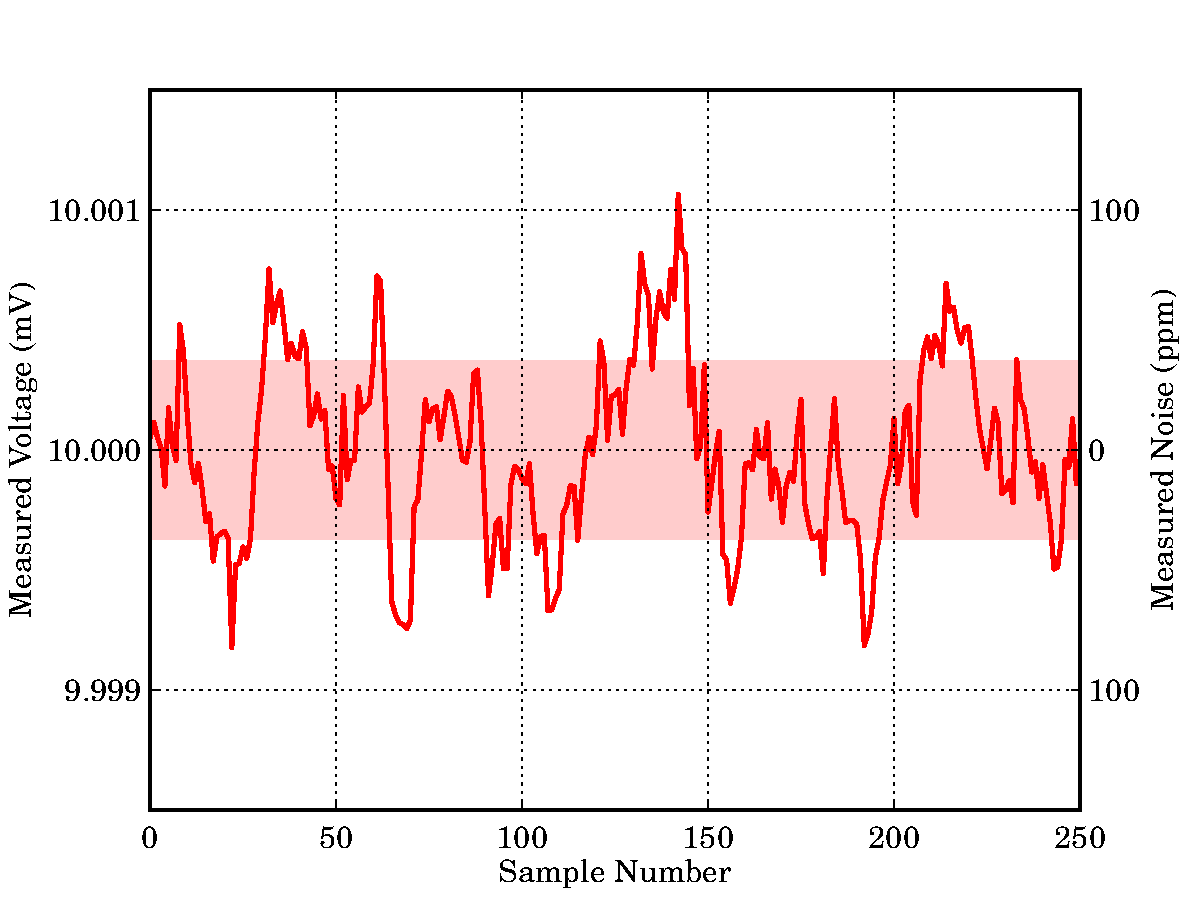
\includegraphics[width = 0.95\textwidth]{figures/RTD_currGen_jitter}
\caption[Jitter from initial, custom-made current bias system.]{Jitter measured from custom-made current bias generator. The input voltage to the system was set such that a current of $10~\mathrm{\upmu A}$ flowed through the $1~\mathrm{k\Omega}$ resistor (which took the place of the device under test). The voltage across the resistor was measured using a trusted data acquisition system. The primary vertical axis shows this voltage (which was expected to be $10~\mathrm{mV}$); the secondary vertical axis shows the jitter or noise about the expected value, in terms of noise parts per million; the shaded region shows the standard deviation of the noise about the expected value.}
\label{fig:RTD_currGen_jitter}
\end{center}
\end{figure}
\par 
Figure~\ref{fig:RTD_currGen_jitter} shows the jitter measured for the current generator which replaced the Keithley unit. The measured peak-to-peak jitter for this system was $200~\mathrm{ppm}$, which corresponded to a maximum variation of $1~\mathrm{\upmu V}$ from the expected value. While this value is approximately twice what was measured in Section~\ref{ssec:bias_prelim} for the Keithley unit (illustrated in Figure~\ref{fig:Keithley220_jitter}), this level was still deemed to be acceptable for \gls{acr:IV} characterisation.

\begin{figure}[t]
\begin{center}
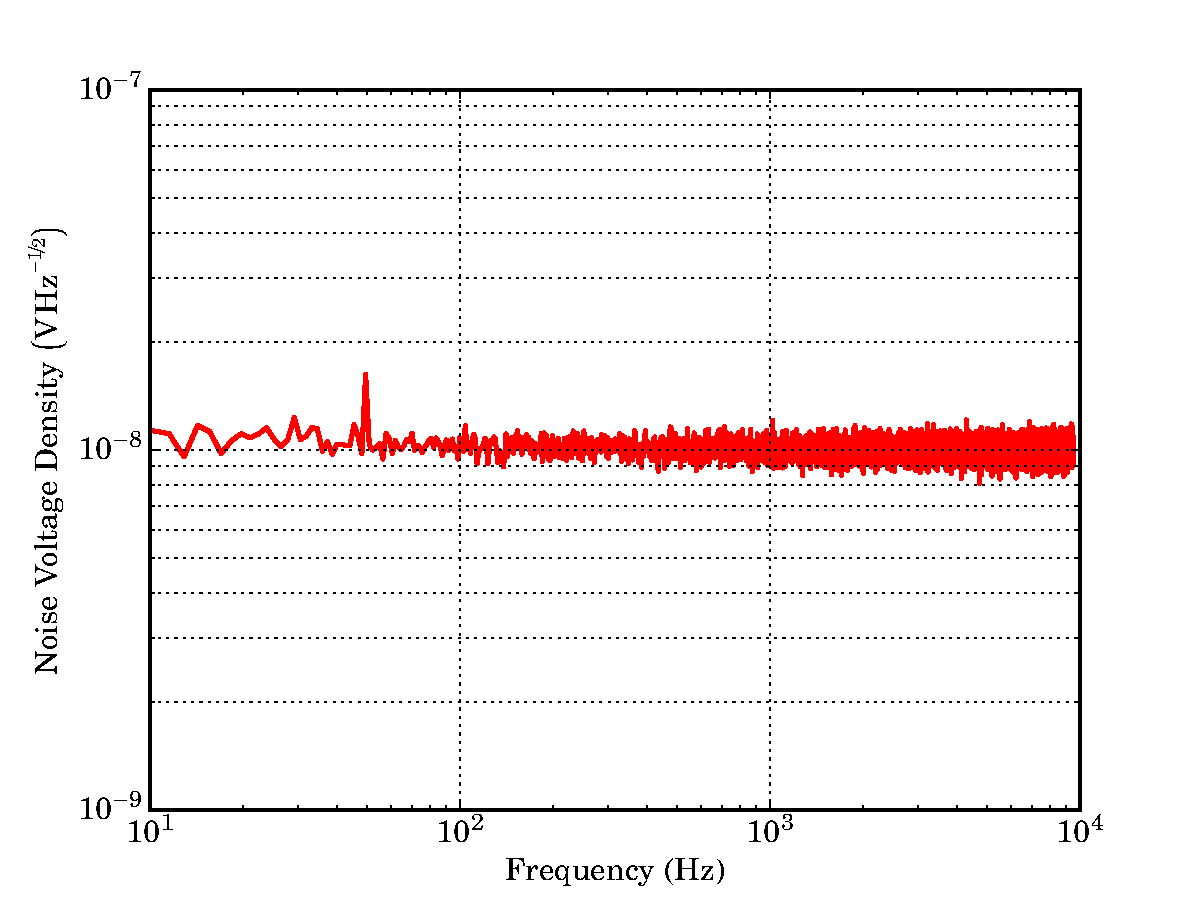
\includegraphics[width = 0.95\textwidth]{figures/RTD_currGen_noise}
\caption[Noise spectrum from original bias generator system, used in conjunction with the initial amplifier.]{The noise spectrum measured across a $1~\mathrm{k\Omega}$ resistor biased using the custom-made bias generator. When compared to the spectrum measured using the Keithley 220, shown in Figure~\ref{fig:Keithley220_noise}, it is clear that the newer system showed very little contamination of this signal.}
\label{fig:RTD_currGen_noise}
\end{center}
\end{figure}
\par 
The noise spectrum measured across a resistor, biased using the newer current generator, is shown in Figure~\ref{fig:RTD_currGen_noise}. When compared to the corresponding measurement in Section~\ref{ssec:readout-prelim} for the Keithley 220 (Figure~\ref{fig:Keithley220_noise}), it is noted that the noise spectrum measured here is much cleaner; there are far fewer noise tones present and the two clusters of tones seen at higher frequencies in Figure~\ref{fig:Keithley220_noise} are no longer present. In fact, the only undesired feature present within the spectrum is the tone at $50~\mathrm{Hz}$, this was due to the $50~\mathrm{Hz}$ variation of the mains power. The white noise level measured in this test was $10~\mathrm{nV\,Hz}^{-\nicefrac{1}{2}}$ compared to a minimum value of $30~\mathrm{nV\,Hz}^{-\nicefrac{1}{2}}$ (rising to over $70~\mathrm{nV\,Hz}^{-\nicefrac{1}{2}}$) for the Keithley unit.  In fact, when the noise spectrum shown in Figure~\ref{fig:RTD_currGen_noise} is compared to the measurement made with the input of the amplifier shorted (Figure~\ref{fig:Keithley220_noise}), it is clear that the two compare extremely favourably. This showed that this measurement was limited by the internal noise generated by the readout amplifier (as shown in Section~\ref{ssec:readout-prelim}).
\par 
From these tests, it was clear that the revised biasing system offered a notable overall improvement when compared to the Keithley 220. Despite there being a decrease in the stability of the bias signal produced, the improvements to noise spectrum and the resulting reduction in unwanted power dissipated across the device under test, meant that this system was used for the preliminary testing of CEB devices.

\section{Final Testing System} \label{sec:Final_Readout}
\subsection{Reason for Replacement}\label{ssec:Final_Readout_Reasons}
Despite having reached a stage where the initial readout system was performing as well as could have been expected of it, it became clear, as the testing of devices progressed, that its limitations were prohibiting the full characterisation of devices. When compared to list of desirable features for the readout system (as defined in Section~\ref{ssec:readout_requirements}), neither the second nor third points were met. That is to say that measurements of noise spectra were limited by the amplifier's own internal noise and that the amplifier did not offer sufficient bandwidth to allow the response speed of a detector to be measured.
\par 
For these reasons, it was decided to replace the initial readout amplifier and bias generator, which had been constructed from non-optimised components and designs already existing within the department, with a new specifically designed system. This system would continue to offer a bias generator similar to the one described in Section~\ref{ssec:RTD_bias_changes&advantages} but with the added feature of being able to internally supply the voltage input to the bias generator; this feature was desirable, as it would offer an ultra-low noise DC bias, albeit at the slight cost of functionality.\footnote{Since this ultra-low noise level was only required when measuring noise spectra, the system could still be used in a way similar to the method described in Section~\ref{ssec:RTD_bias_changes&advantages} without any loss of functionality.}

\subsection{Final Readout System}\label{ssec:final_readout}
\begin{figure}[t]
\begin{center}
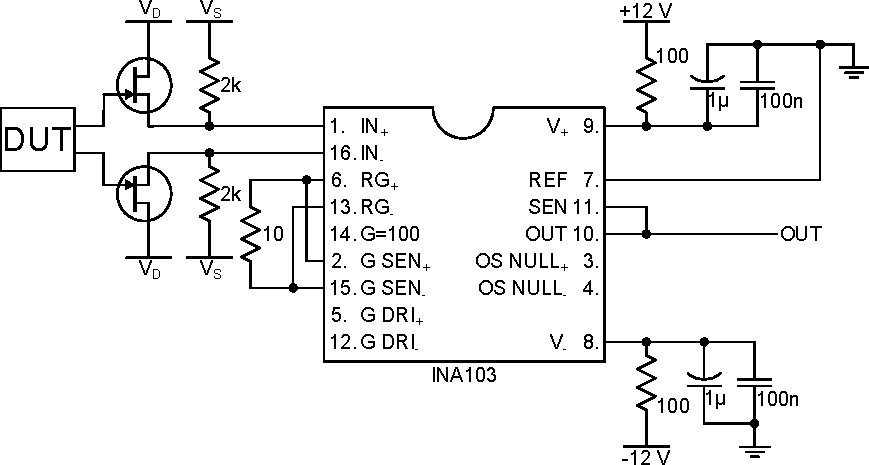
\includegraphics[width = 0.95\textwidth]{figures/final_amp}
\caption[Final voltage Readout Amplifier]{Final amplifier used for measuring voltage across devices. As opposed to the previous system (Figure~\ref{fig:rtd_readout_amp}), only one amplifier stage was used: the Texas Instruments INA103 amplifier, which was configured to offer a gain of $600$. In addition to the amplifier, a matched pair of JFETs were used as source followers. This improved coupling to the amplifier by offering a low output impedance. It also isolated the amplifier from the device being measured, thus resulting in a lower noise level.}
\label{fig:finalAmp}
\end{center}
\end{figure}

Figure~\ref{fig:finalAmp} shows the amplifier used for the final stages of testing silicon cold-electron bolometers. The main amplification was performed by a INA103 chip manufactured by Texas Instruments. However, in order to provide a low-impedance input to the amplifier, as well as isolating the device under test from the amplifier circuitry, a matched pair of \gls{acr:JFET} were used to create a differential source follower to act as the input of the amplifier. 
\par 
One disadvantage of this configuration was that the addition of the \gls{acr:JFET} source followers meant that an offset voltage was added at the input of the amplifier. As explained by \citet[chap. 2]{HorowitzHill1989}, this is the result of inconsistencies in the current produced by a given voltage across the gate and source of the JFET. The reason for these inconsistencies is due to this parameter being poorly controlled in the manufacture of JFETs. This could have been addressed by including a second JFET, matched to the existing JFET, that acted to vary the source voltage to the first JFET, such that there would have been no voltage offset at the output (which would have been at the drain terminal of this second JFET). This modification was not however applied, since the differential input to the amplifier already necessitated  that the two JFETs be matched and the increase to quad-matched JFETs was prohibitively expensive for a non-critical improvement.
\par 
The preliminary testing had indicated that the previous amplifier's gain of $1000$ was possibly excessive. To this end, it was decided that a lower gain, of approximately $600$, would be used in this case. The \textcite{INA103DS} does not provide a table of the required resistance across the gain setting pins to achieve this value, there is however the equation for the gain, $G$:
\begin{align}
G &= 1 + \frac{6000}{R_{\mathrm{G}}}\, , \label{eqn:INA103gain}
\intertext{where $R_{\mathrm{G}}$ is the value of the gain setting resistor required to achieve a gain of $G$. Thus, the value of the resistor required for a gain of $600$ could be found as:}
R_{G=600} &= \frac{6000}{600 - 1}\, ,\\
R_{G=600} &\approx{10}\, . \label{res:finalAmpGain}
\end{align}

\begin{figure}[t]
\begin{center}
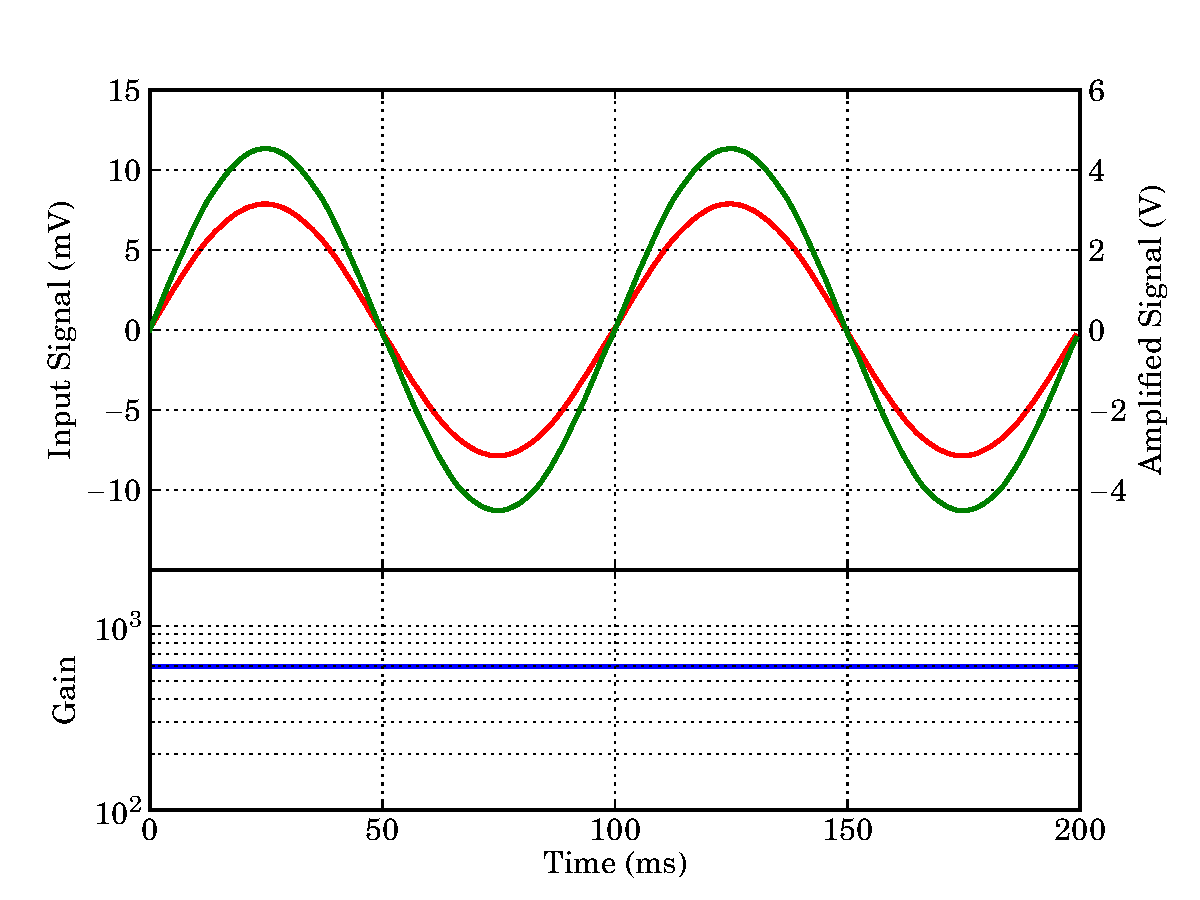
\includegraphics[width = 0.95\textwidth]{figures/final_amp_gain}
\caption[Gain measurement of final amplifier]{Gain measurement for the amplifier used in the final test of silicon cold-electron bolometers. As in Section~\ref{ssec:readout-prelim}, a $10~\mathrm{Hz}$ sinusoidal signal was supplied to the input of the amplifier and the output measured. Upper plot -- Input signal (red, primary vertical axis) compared to the output of the amplifier (greed, secondary vertical axis). Lower plot -- Gain measured from the ratio of the output and input signals.}
\label{fig:finalAmp_gain}
\end{center}
\end{figure}
\par 
As had been performed for the previous amplifier (Section~\ref{ssec:readout-prelim}), a sinusoidal signal was split, with one feed supplied to the input of the amplifier and the other, along with the output of the amplifier, measured using a digital oscilloscope. The gain of the amplifier could then be calculated by simply taking the ratio of these two values. The results of these measurements are shown in Figure~\ref{fig:finalAmp_gain} where it can be seen that, for an input signal with an amplitude of $7.5~\mathrm{mV}$, there is uniform amplification at all amplitudes and the gain factor was 600.
\begin{figure}[t]
\begin{center}
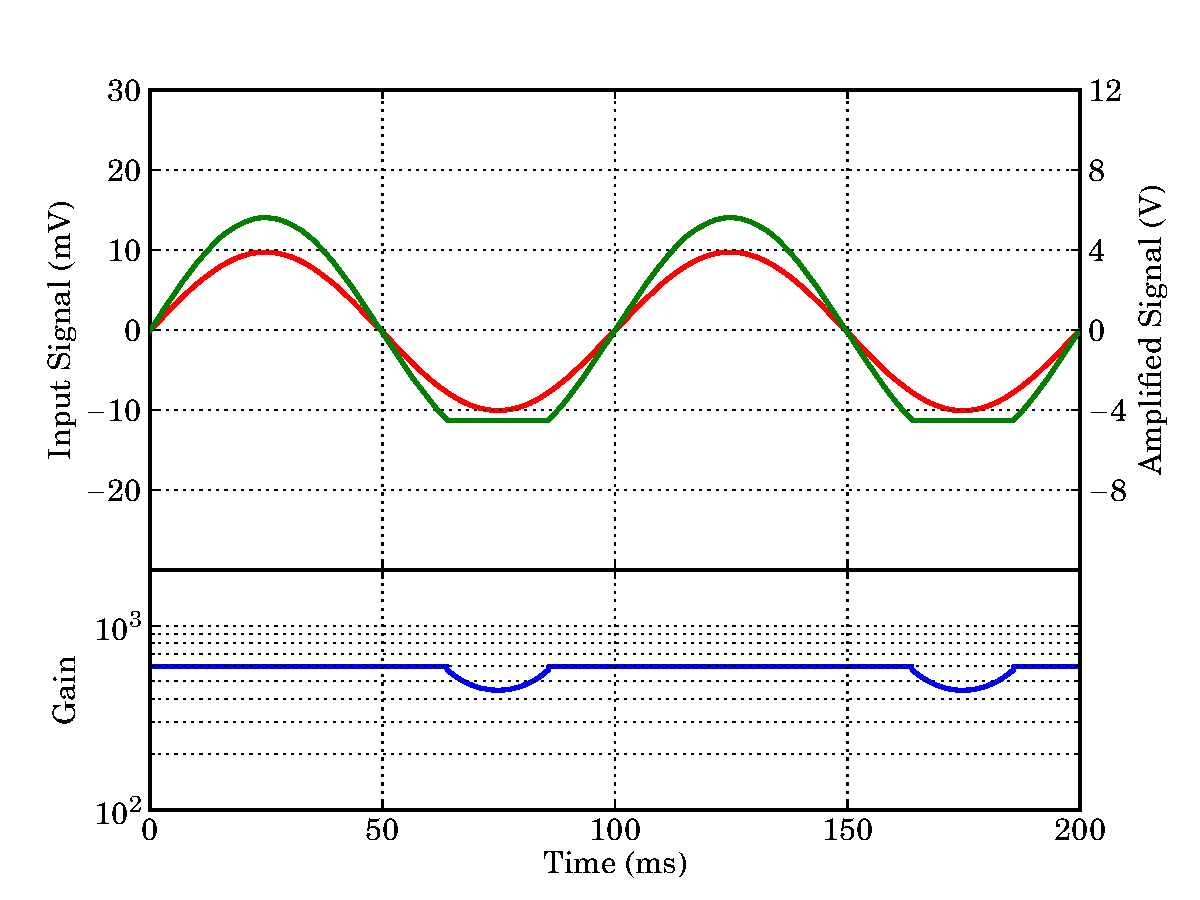
\includegraphics[width = 0.95\textwidth]{figures/final_amp_gain_limit}
\caption[Asymmetric limit to input of the final amplifier]{When the input to the final amplifier was increase above an amplitude of $7.5~\mathrm{mV}$, an asymmetric response was noted. While positive signal continued to be amplified, by a gain factor of 600, the negative signal with the same magnitude became limited to a certain minimum value. Upper plot -- Input signal (red, primary vertical axis) compared to the output of the amplifier (green, secondary vertical axis). Lower plot -- Gain measured from the ratio of the output and input signals.}
\label{fig:finalAmp_gain_limit}
\end{center}
\end{figure}
\par 
The addition of the \gls{acr:JFET} source followers caused a further complication with this amplifier. Figure~\ref{fig:finalAmp_gain_limit} shows what happened when the amplitude of the input signal to the amplifier was increased above the $7.5~\mathrm{mV}$ illustrated in Figure~\ref{fig:finalAmp_gain}. In Figure~\ref{fig:finalAmp_gain_limit}, it is clear that there is a lower limit to the output voltage (green line shown on the secondary vertical axis) of approximately $-4.5~\mathrm{V}$. In order to understand the origin of this limit and any significance it might have had on testing, it is important, as always, to fully understand how these data were collected. As has already been mentioned, the presence of the JFET source followers resulted in an (undesired) DC voltage offset to the input of the INA103 amplifier. When measured, this offset was found to be $-6.59~\mathrm{V}$ at the output of the amplifier (or $-11~\mathrm{mV}$ at the input). In order to correct for this simply in the measurement, the input of the digital oscilloscope (which was used for all the measurements in this section) was set to AC-coupling. This meant that values which were recorded as $0~\mathrm{V}$ in the AC-coupled measurement corresponded to an output voltage of $-6.59~\mathrm{V}$ from the amplifier. The \textcite{INA103DS} explains that the amplifier is capable of a maximum voltage output range of $\pm 11~\mathrm{V}$. By dividing by the gain of the amplifier ($600$ in the configuration used), it was possible to calculate the range of input voltages to the amplifier, for which a correctly amplified output was attainable (i.e. those which corresponded to an output of less than $\pm 11~\mathrm{V}$); this was found to be $\pm 18.\dot{3}~\mathrm{mV}$. As explained earlier however, the JFET source follower used resulted in an offset voltage of $-11~\mathrm{mV}$ at the input of amplifier. When this was subtracted from the input range of the amplifier, the effective range of input voltages, $V_{\mathrm{input_{eff}}}$, was found to be
\begin{align}
V_{\mathrm{input_{eff}}} &= V_{\mathrm{input}} - V_{\mathrm{offset}}\, , \label{eqn:amp_input_range}\\
&= \pm 18.3~\mathrm{mV} - -11.0~\mathrm{mV}\, , \\  
&= ^{+29.3}_{-\hphantom{2} 7.3}~\mathrm{mV} \, . \label{res:finalAmp_input_range}
\end{align}
While this result had the advantage of meaning the amplifier system had an increased range for positive signals, there was a severe restriction placed on the amplifier's ability to handle negative signals. Fortunately, the required measurable input voltage range for testing SiCEB devices was only of the order of $\pm 1~\mathrm{mV}$, with few circumstances existing where signals of greater magnitude were measured and none that would require measuring to as low as $7.3~\mathrm{mV}$ across the device. For comparison, the previous amplifier's input range, which did not suffer from any asymmetry, was $\pm 13~\mathrm{mV}$.
\par 
Since the restricted range of input voltage did not, in fact, affect the amplifier's suitability for the measurements being undertaken, it was decided that there was no need to address this, despite it being non-ideal. As previously mentioned, the DC offset due to the JFET could have been removed via the addition of a second JFET on each input, if necessary.
\begin{figure}[ht]
\begin{center}
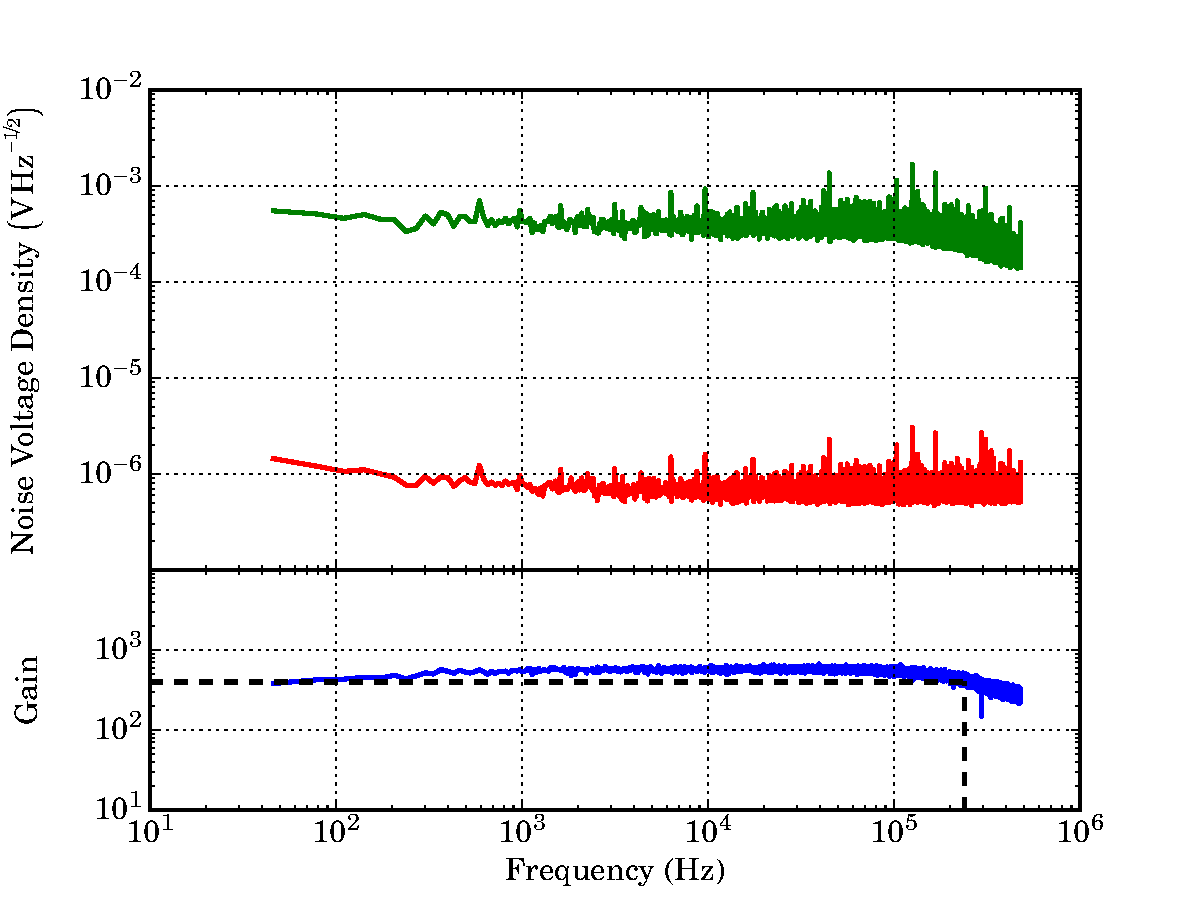
\includegraphics[width = 0.95\textwidth]{figures/final_amp_BW}
\caption[Bandwidth measurement of final amplifier]{Bandwidth measurement of final amplifier. A white noise signal (red trace) was generated and supplied to the amplifier whose output (green trace) was also monitored. The ratio of these two (the gain---blue trace) was also calculated.}
\label{fig:finalAmp_BW}
\end{center}
\end{figure}
\par 
In order to measure the 3-dB bandwidth of this amplifier, the same measuring procedure was used as for the initial amplifier (described fully in Section\ref{ssec:readout-prelim}). A signal generator was used to create a white noise signal which was input to the amplifier. The output of the amplifier, along with the output of the signal generator, were monitored using a digital oscilloscope. To measure the bandwidth of the amplifier, the ratio of the input of the amplifier to its output (its gain) was measured; the results of this are shown in Figure~\ref{fig:finalAmp_BW}. As explained by Equation~\ref{eqn:3dBV}, the edge of the $3~\mathrm{dB}$ bandwidth corresponds to the frequency at which the gain has fallen by a factor of $\sqrt{2}$. The lower plot in Figure~\ref{fig:finalAmp_BW}, shows the measured gain with the dashed lines illustrating the $3~\mathrm{dB}$ level, which was a gain of $424$, and the corresponding frequency was found to be $240~\mathrm{kHz}$\label{res:final_amp_BW}. This shows that the amplifier offered a substantial improvement compared to its predecessor, whose 3-dB bandwidth was equal to $55~\mathrm{kHz}$ (calculated on Page~\pageref{res:RTD_amp_BW}). Although the \textcite{INA103DS} does not provide a figure for the expected bandwidth of the amplifier when operating with a gain of 600, it does provide values of $6~\mathrm{MHz}$ and $800~\mathrm{kHz}$ for gains of 1 and 100 respectively, this seems to indicate that the value of $240~\mathrm{kHz}$, at a gain of 600, is to be expected.
\begin{figure}[t]
\begin{center}
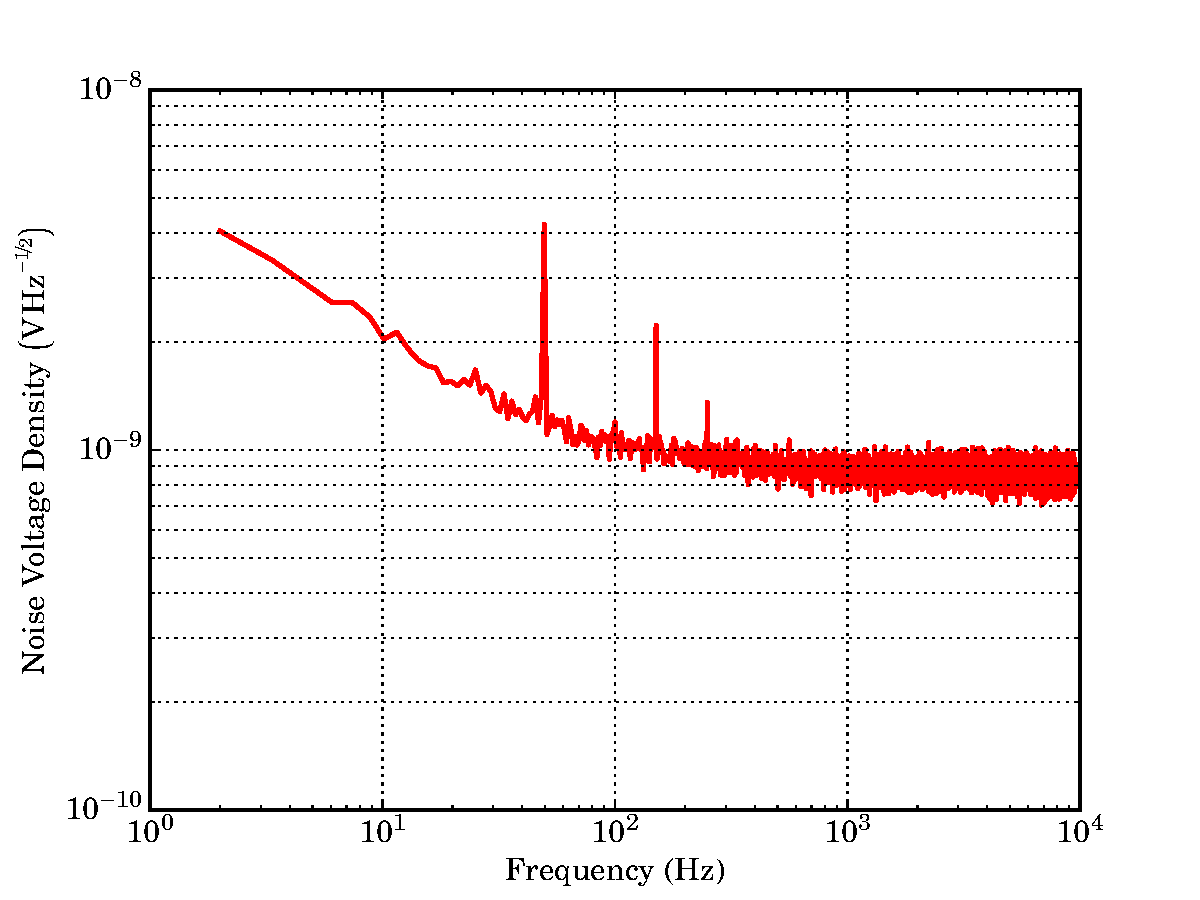
\includegraphics[width = 0.95\textwidth]{figures/final_amp_IRN}
\caption[Measurement of the internal noise, referred to the input, for the final amplifier.]{Measurement of the internal noise, referred to the input, for the final amplifier. This was measured with a shorted input of the amplifier.}
\label{fig:finalAmp_IRN}
\end{center}
\end{figure}
\par 
Figure~\ref{fig:finalAmp_IRN} shows the measurement of the internal noise of the final amplifier. This was measured with the input to the amplifier (the gates of the two JFET source followers) shorted such that there was a differential signal of $0~\mathrm{V}$ at the input of the amplifier. The output of the amplifier was fed to a digital oscilloscope, which computed the Fourier transform of the signal. This was then divided by the gain (measured in Figure~\ref{fig:finalAmp_gain}), to give the input-referred internal noise of the amplifier. From Figure~\ref{fig:finalAmp_IRN} it can be seen that the white noise level of this noise spectrum is approximately $1.5~\mathrm{nV\,Hz}^{-\nicefrac{1}{2}}$ and that the spectrum is white from a few hundred hertz up until the end of the measurement at $10~\mathrm{kHz}$. 
\par 
When compared to the corresponding measurement for the previous amplifier, shown in Figure~\ref{fig:RTD_amp_IRN}, two key differences are immediately apparent. Firstly, the newer amplifier has a substantially lower noise level, with the white noise floor of he previous amplifier having been $10~\mathrm{nV\,Hz}^{\nicefrac{-1}{2}}$, compared to the newer device's level of $850~\mathrm{pV\,Hz}^{\nicefrac{-1}{2}}$; this notable improvement was the key reason for switching to the newer amplifier. Secondly, there was a more pronounced level of $1/f$ noise visible in the spectrum for the newer amplifier compared to its predecessor. While this increase was indeed undesirable, the \textcite{INA103DS} indicates that this is to be expected for this device and it is worth noting that even when allowing for this additional noise the newer amplifier still offered lower noise at these frequencies than the previous amplifier.
\par 
These two tests showed that the replacement amplifier offered a notable improvement, in all areas, over the initial amplifier used and also showed that despite the newer device having some limitations not present in its predecessor (principally the asymmetric limit to the input voltage, shown in Figure~\ref{fig:finalAmp_gain_limit}), these limitations did not stop it from being fit for the testing required. 
%
\subsection{Final Bias System}\label{ssec:final_bias}
\begin{figure}[t]
\begin{center}
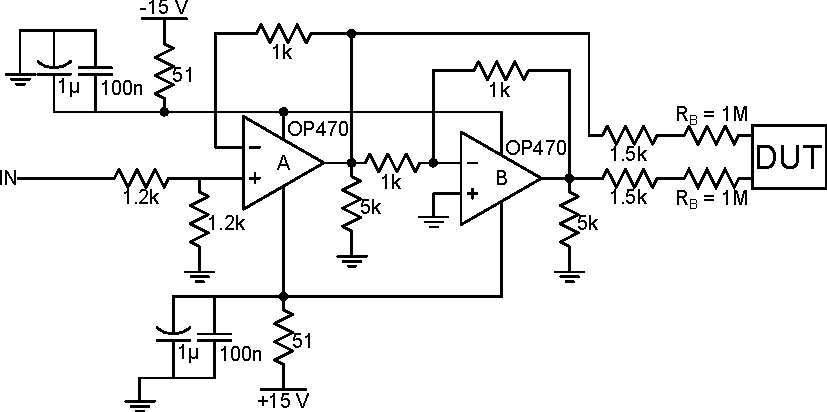
\includegraphics[width = 0.95\textwidth]{figures/final_bias}
\caption[Differential bias generator used with final readout system]{Circuitry used to generate a differential signal used to bias the device under test. The principle is the same as described in Section~\ref{sec:RTD_bias}.}
\label{fig:final_currGen}
\end{center}
\end{figure}
For simplicity, a biasing system, similar to that described in Section~\ref{sec:RTD_bias} (which has been shown to function well), was integrated into this final system. The circuitry for this is shown in Figure~\ref{fig:final_currGen}. The only difference in operation between this circuit and the system used previously was the relation between the input signal and the differential output. For the previous system, this was $1:2$, meaning for an input of $1~\mathrm{V}$, a differential signal of $2~\mathrm{V}$ was output (as explained on Page~\pageref{res:RTDVbias}). The key difference here was that, although both of the OP470 amplifiers (manufactured by Analog Devices and, in fact, housed within a single package) were configured to provide a gain factor of unity, an additional potential was included at the input of the first amplifier. This divider (the two $1.2~\mathrm{k\Omega}$ resistors seen in Figure~\ref{fig:final_currGen}) acted to reduce the input of the first amplifier by a factor of two. This meant that the output of each of the amplifiers was equal to one half of the input voltage, thus the total differential voltage at the output was the same as the input voltage. As in the previous case, the device was biased via a pair of $1~\mathrm{M\Omega}$ biasing resistors and the biasing current can be calculated similarly to the method on Page~\pageref{eqn:diffBiasGen}. For this system, using Equation~\ref{eqn:diffBiasGen}, the biasing voltage $V_{\mathrm{bias}}$ was given simply by:
\begin{align}
V_{\mathrm{bias}} &= V_{\mathrm{in}} \, ,\label{eqn:finalVbias}
\intertext{where $V_{\mathrm{in}}$ was the input voltage to the bias generator. This meant that the biasing current, $I_{\mathrm{bias}}$, across the device under test was calculated as:}
I_{\mathrm{bias}} &= \frac{V_{\mathrm{R}}}{2 R_{\mathrm{bias}}} \,, \tag{\ref{eqn:OhmsRbias} revisited}
\intertext{where $V_{\mathrm{R}}$ is again the voltage dropped across the biasing resistors and, given the result shown in Equation~\ref{eqn:finalVbias}, was calculated by:}
V_{\mathrm{R}} &= V_{\mathrm{in}} - V_{\mathrm{DUT}} \, ,\label{eqn:RbiasVfinal} 
\intertext{where $V_{\mathrm{DUT}}$ is the voltage measured across the device under test. Finally, combining this with Equation~\ref{eqn:OhmsRbias} gave the final relation for the biasing current:}
R_{\mathrm{bias}} &= \frac{V_{\mathrm{in}} - V_{\mathrm{DUT}}}{2 R_{\mathrm{bias}}} \, . \label{res:finalIbias}
\end{align}
\begin{figure}[t]
\begin{center}
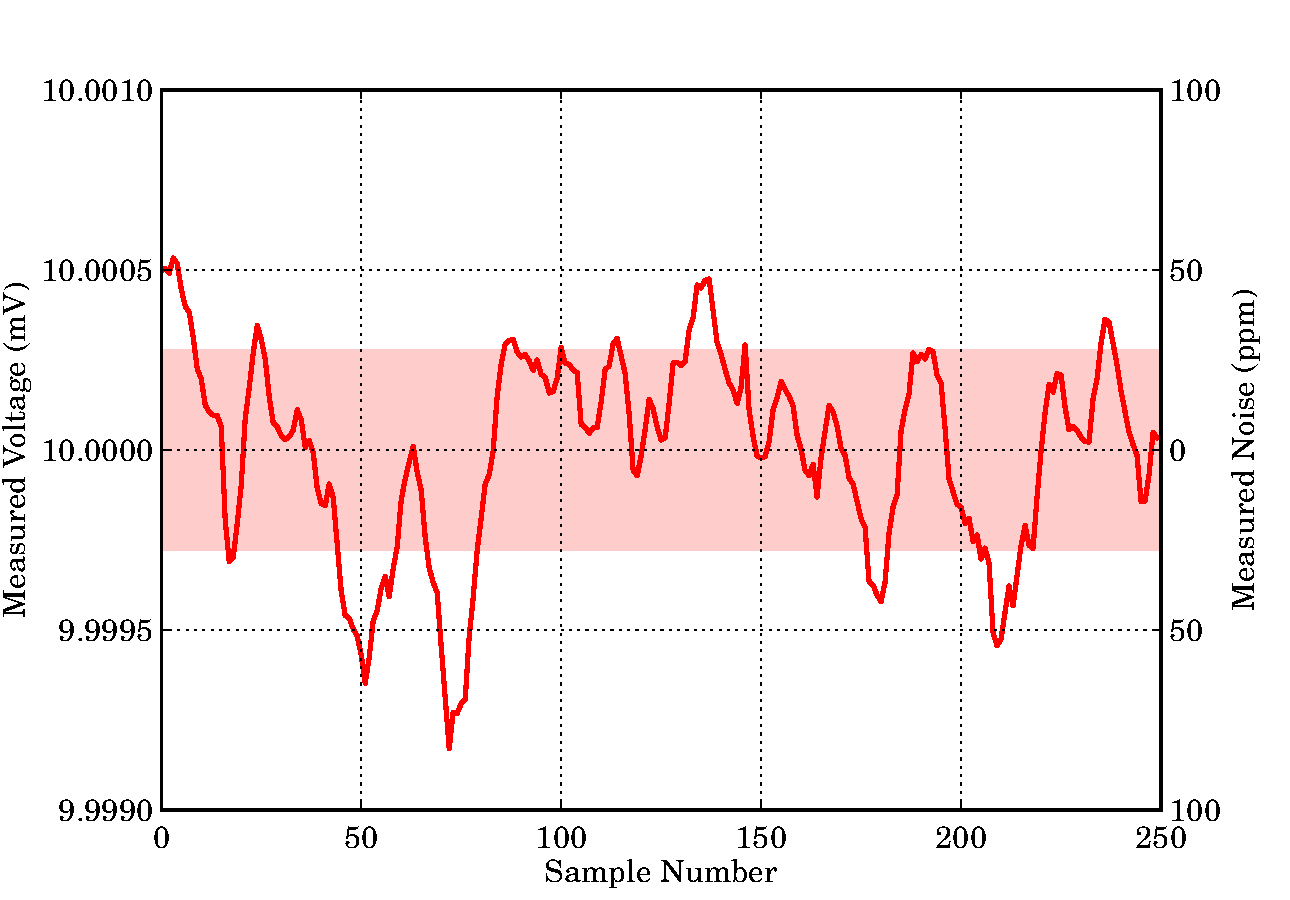
\includegraphics[width = 0.95\textwidth]{figures/final_bias_jitter}
\caption[Measurement of jitter from the bias generator used in conjuncture with the final readout system.]{Measurement of jitter from the bias generator used with the final readout amplifier. The generator was configured to produce a biasing current of $1~\mathrm{\upmu A}$, which was driven across a $10~\mathrm{k\Omega}$ resistor.}
\label{fig:final_currGen_jitter}
\end{center}
\end{figure}
\par 
As for the previous biasing systems, it was important to measure the jitter in the current produced. This was preformed by configuring the bias generator to produce a current of $1~\mathrm{\upmu A}$, which was driven across a $10~\mathrm{k\Omega}$ resistor.\footnote{The input voltage to the bias generator for this measurement was provided by using the system's on-board voltage (controlled through a potential divider) rather than an external source.} This meant that the expected voltage measured across the resistor, according to Ohm's Law, was $10~\mathrm{mV}$. Figure~\ref{fig:final_currGen_jitter} shows the results of this measurement. The maximum variation from the expected value was $800~\mathrm{nV}$ which corresponded to a peak-to-peak jitter of $160~\mathrm{ppm}$. While this was still not as low as the jitter measured for the Keithley 220 unit, which was $110~\mathrm{ppm}$, it was, in fact, an improvement on the value of $200~\mathrm{ppm}$ which was measured for the previous bias generator in Section~\ref{ssec:RTD_bias_performance}. Since the jitter of the previous system had caused no problems, there was no reason to conclude that any issue would be presented here.
\begin{figure}[tb]
\begin{center}
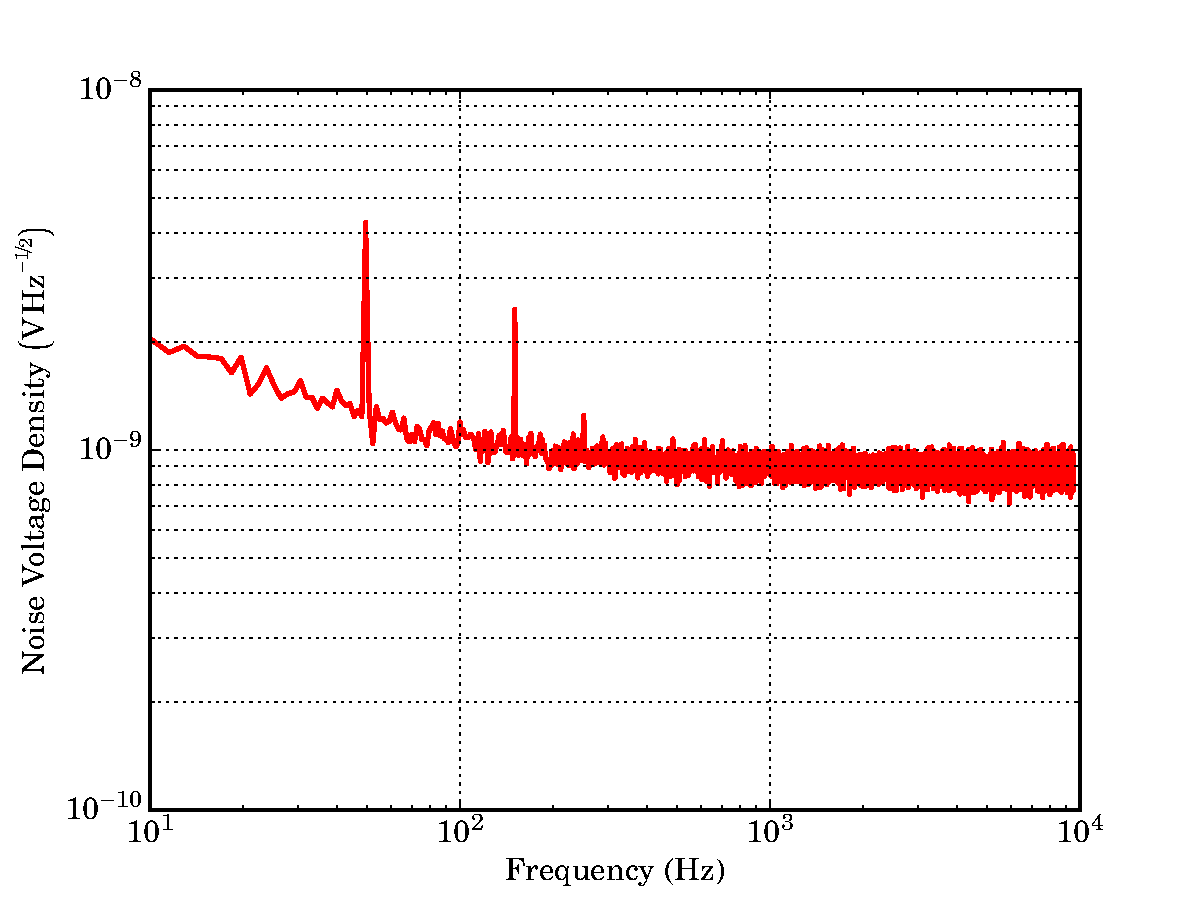
\includegraphics[width = 0.95\textwidth]{figures/final_bias_noise}
\caption[Noise measurement for bias generator used in conjuncture with the final readout system.]{Noise measurement for the bias generator used in conjunction with the final readout system. A low value resistor $\left(\approx 10~\mathrm{\Omega}\right)$ was placed across the output generator and the amplifier was used to amplify the signal. The output of the amplifier was read by a digital oscilloscope which computed the noise spectrum.}
\label{fig:final_currGen_noise}
\end{center}
\end{figure}
\par
Figure~\ref{fig:final_currGen_noise} shows the noise spectrum, measured using the amplifier described in Section~\ref{ssec:final_readout}, for a device (a low resistance resistor) biased by the system shown in Figure~\ref{fig:final_currGen}. Comparison between this figure and the noise spectrum shown in Figure~\ref{fig:finalAmp_IRN} shows that the dominating noise is from the internal processes in the amplifier and that the bias generator did not contribute any additional noise to this measurement. This is that same as had been found for the previous bias generator system and is not a surprise considering the similarities, in operational principle, between the two systems.

\section{Cross-Correlated Noise Measurement}\label{sec:cross_col_noise}
Despite the improved (lower) noise limit of the system detailed in Section~\ref{sec:Final_Readout}, this system was, at best, only able to measure noise generated within a device at optimum bias\footnote{The dependance of various noise sources on the bias, or more correctly the bias dependant responsivity, is explained in Section~\ref{sec:theory-NEP}.}. To allow a full study of the sensitivity of a device, it was important to be able to measure the noise in the device over the greatest possible range of biases. To this end, an innovative solution was devised to reduce the noise level of the readout system. This was to split the voltage readout of the device between two identical amplifiers and then to use a computer to cross-correlate the output of these to effectively remove the noise contribution of the amplification.

\subsection{Convolution}\label{ssec:convultion}
The convolution of two signals or functions is a third function whose amplitude is given by the area overlap of the functions $f$ and $g$, when one of the functions is reversed and then translated across the other function. Common applications of convolution include: measuring the response function to an impulse function \citep{Callier1978}; in probability, the convolution of two independent variables gives the probability distribution \citep{Hogg2012}; in acoustics and sound-engineering, reverberation is the convolution of an original signal with reflections (echos) from surfaces \citep{Begault2007}; in signal processing, a weighted average of a signal is a convolution.
\par 
In time-space, the convolution of two functions, $f$ and $g$, is written as $f \ast g$. Mathematically, this is computed by reversing one of these functions such that $f(t) \rightarrow f(t - \tau)$ and is then translated across the other function. This can be written as an integral:
\begin{align}
\left(f \ast g\right)\left(t\right) &\stackrel{\mathrm{def}}{=}  \int_{-\infty}^{\infty} f\left(\tau \right)g\left(t - \tau \right)\,\d\tau \,.
\label{def:convolution}
\intertext{Convolution is commutative so $f \ast g = g \ast f$ or, more completely:}
\left(f \ast g\right)\left(t\right) &\stackrel{\mathrm{def}}{=}  \int_{-\infty}^{\infty} f\left(\tau \right)g\left(t - \tau \right)\,\d\tau\,, 
	\nonumber \\
&=\int_{-\infty}^{\infty} f\left(t-\tau \right) g\left(\tau \right)\,\d\tau \,.
\end{align}
\par 
It is, perhaps, easiest to understand convolution, in the time domain, graphically. This is shown in Figure~\ref{fig:convolution_time}. From this figure, it can be seen that the value of convolution at any time $\tau$ is given by the area overlap of the two functions (shown as the highlighted regions in Figures \ref{fig:conv_t1} to \ref{fig:conv_t5}), when the leading non-zero value of the reversed function ($g\left(t\right)$ in this case) is at $\tau$.
\begin{figure}[p]
\begin{center}
\subfloat[]{
	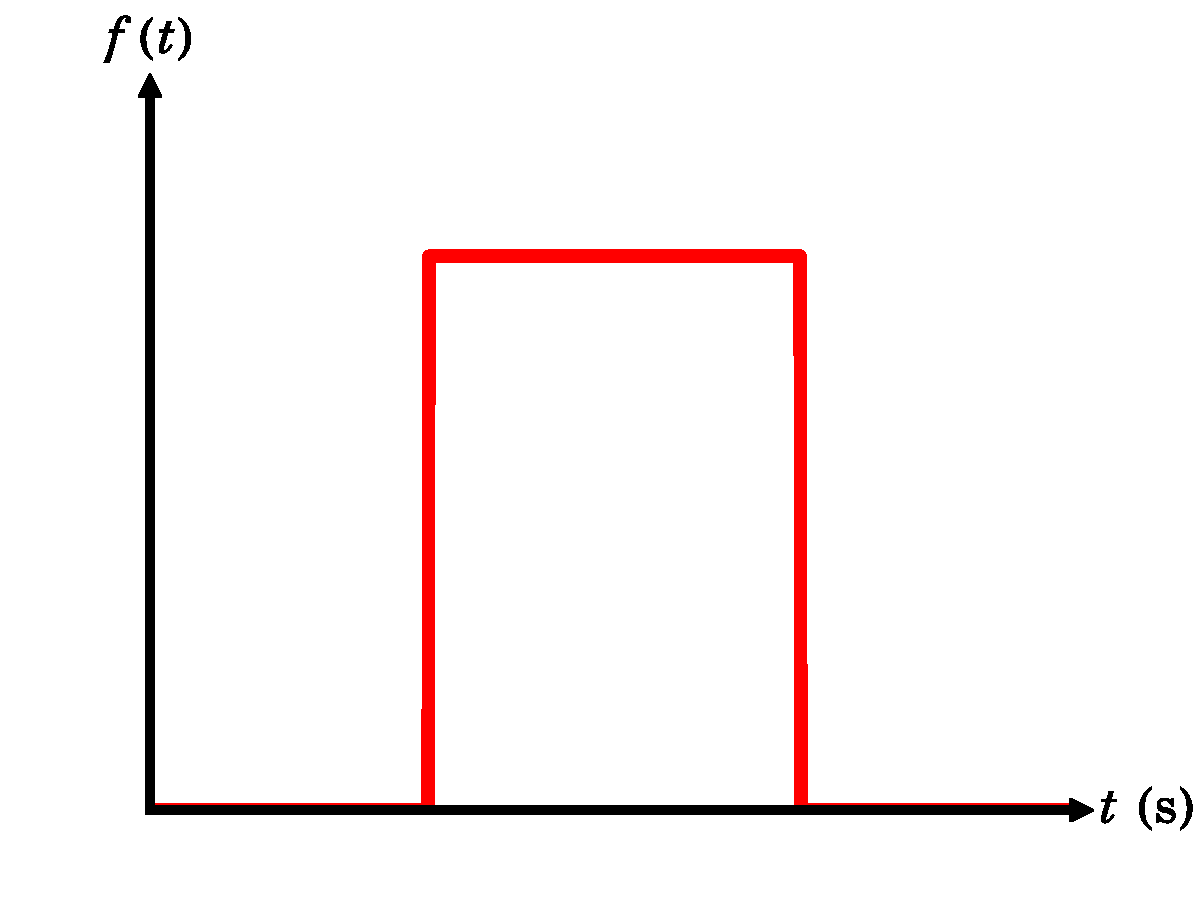
\includegraphics[width=0.32\textwidth]{figures/convolution_f}
	\label{fig:conv_f}
}
\subfloat[]{
	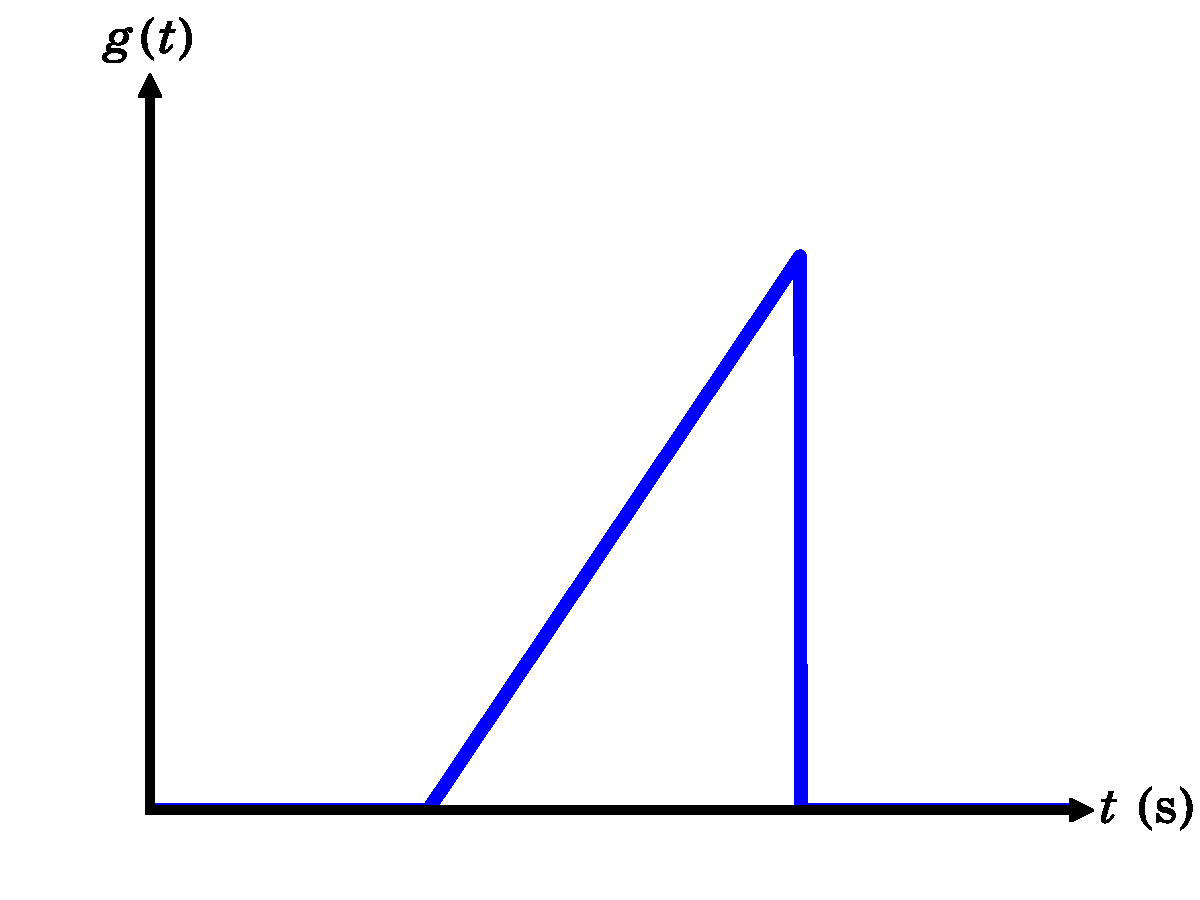
\includegraphics[width=0.32\textwidth]{figures/convolution_g}
	\label{fig:conv_g}
}
\subfloat[]{
	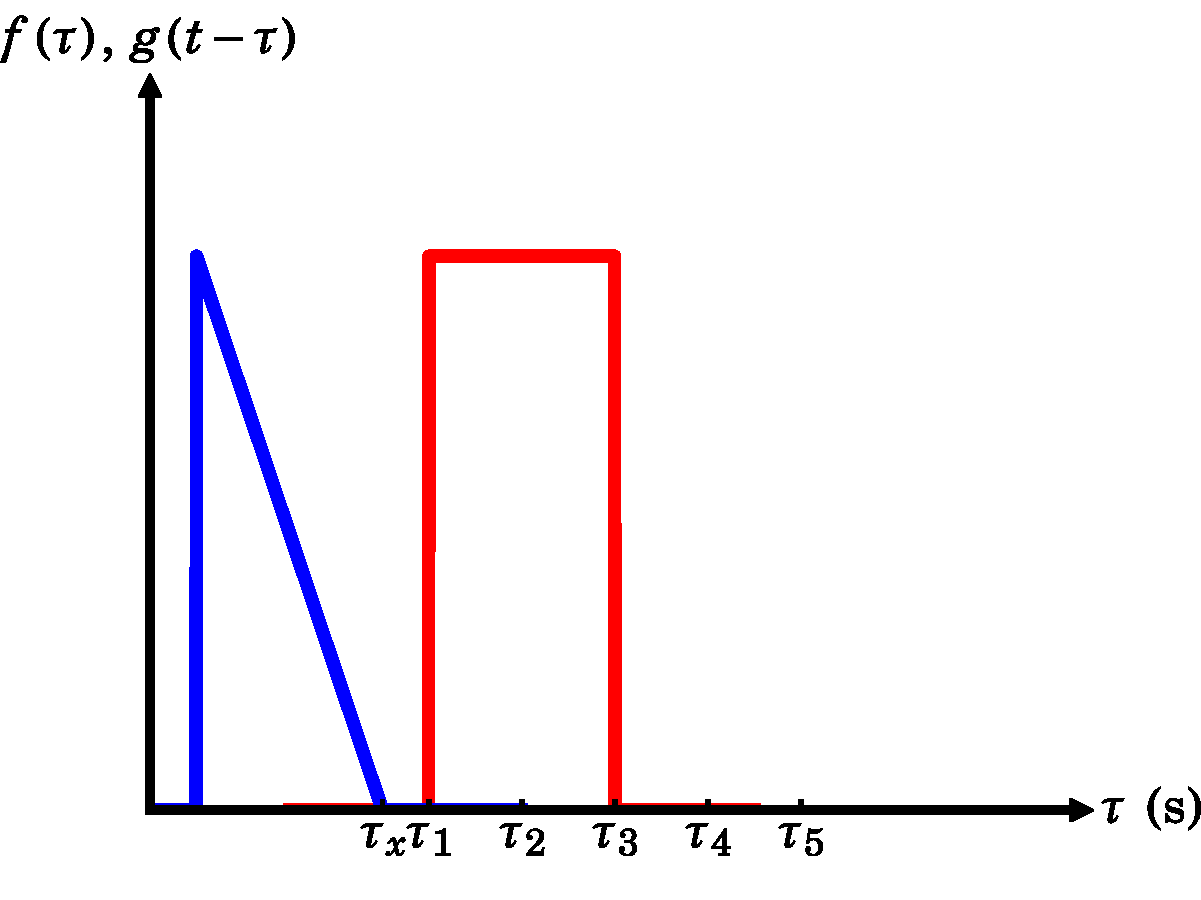
\includegraphics[width=0.32\textwidth]{figures/convolution_tx}
	\label{fig:conv_tx}
}
\\
\subfloat[]{
	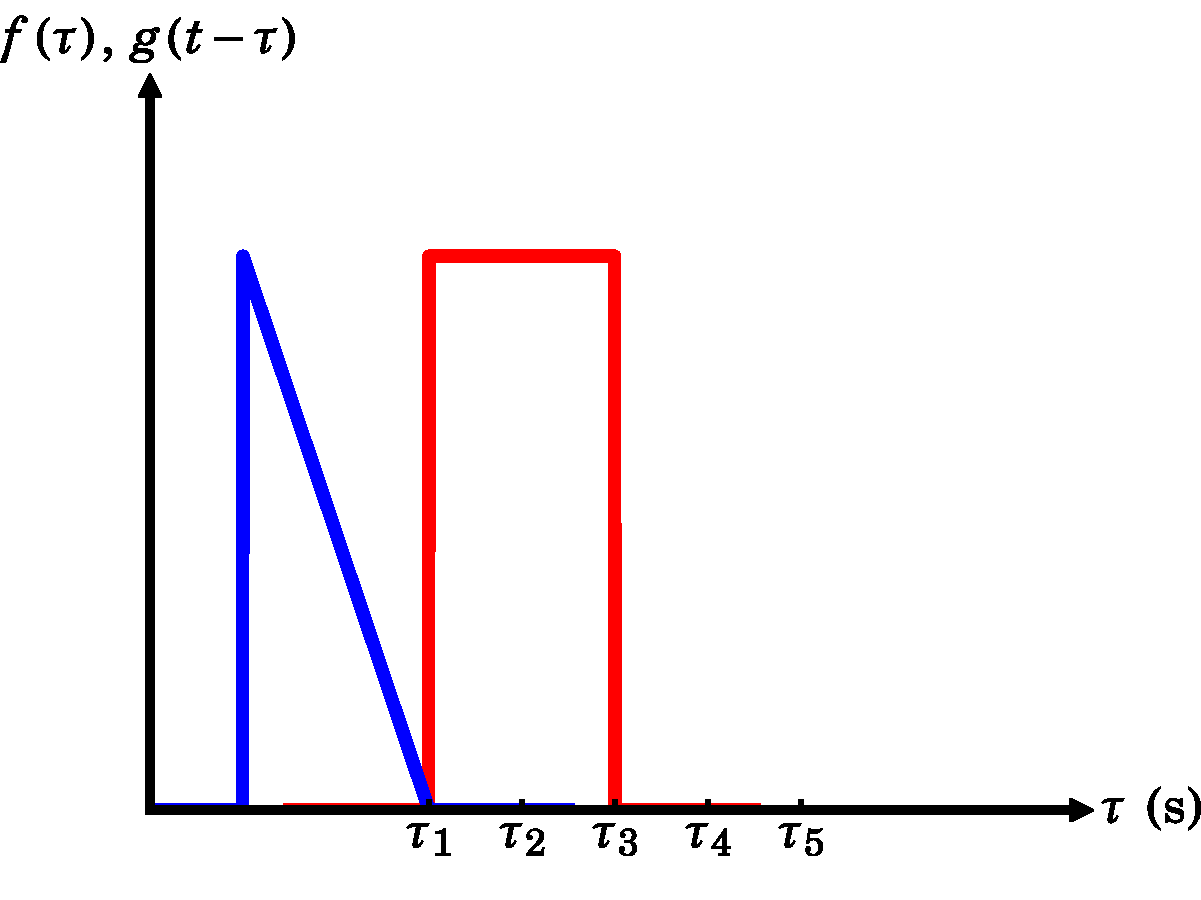
\includegraphics[width=0.32\textwidth]{figures/convolution_t1}
	\label{fig:conv_t1}
}
\subfloat[]{
	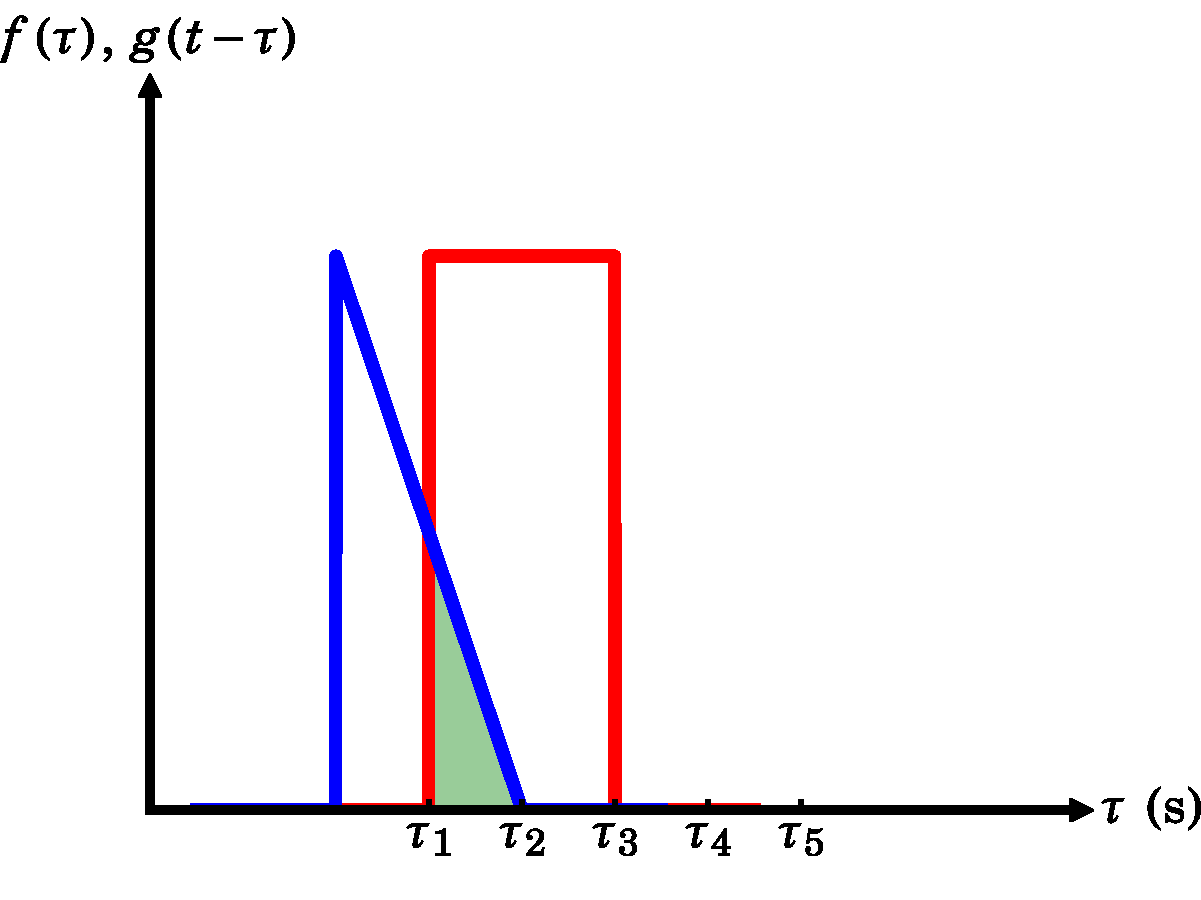
\includegraphics[width=0.32\textwidth]{figures/convolution_t2}
	\label{fig:conv_t2}
}
\subfloat[]{
	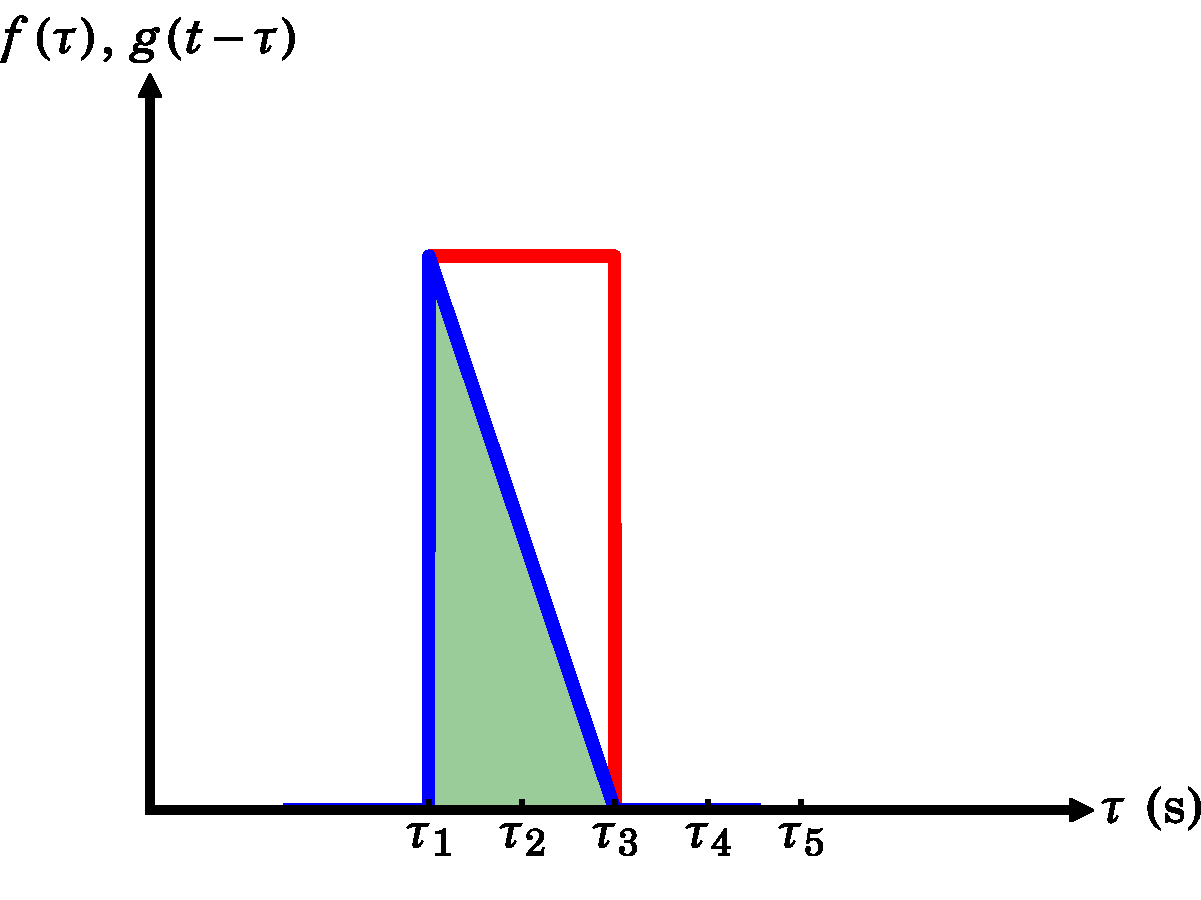
\includegraphics[width=0.32\textwidth]{figures/convolution_t3}
	\label{fig:conv_t3}
}
\\
\subfloat[]{
	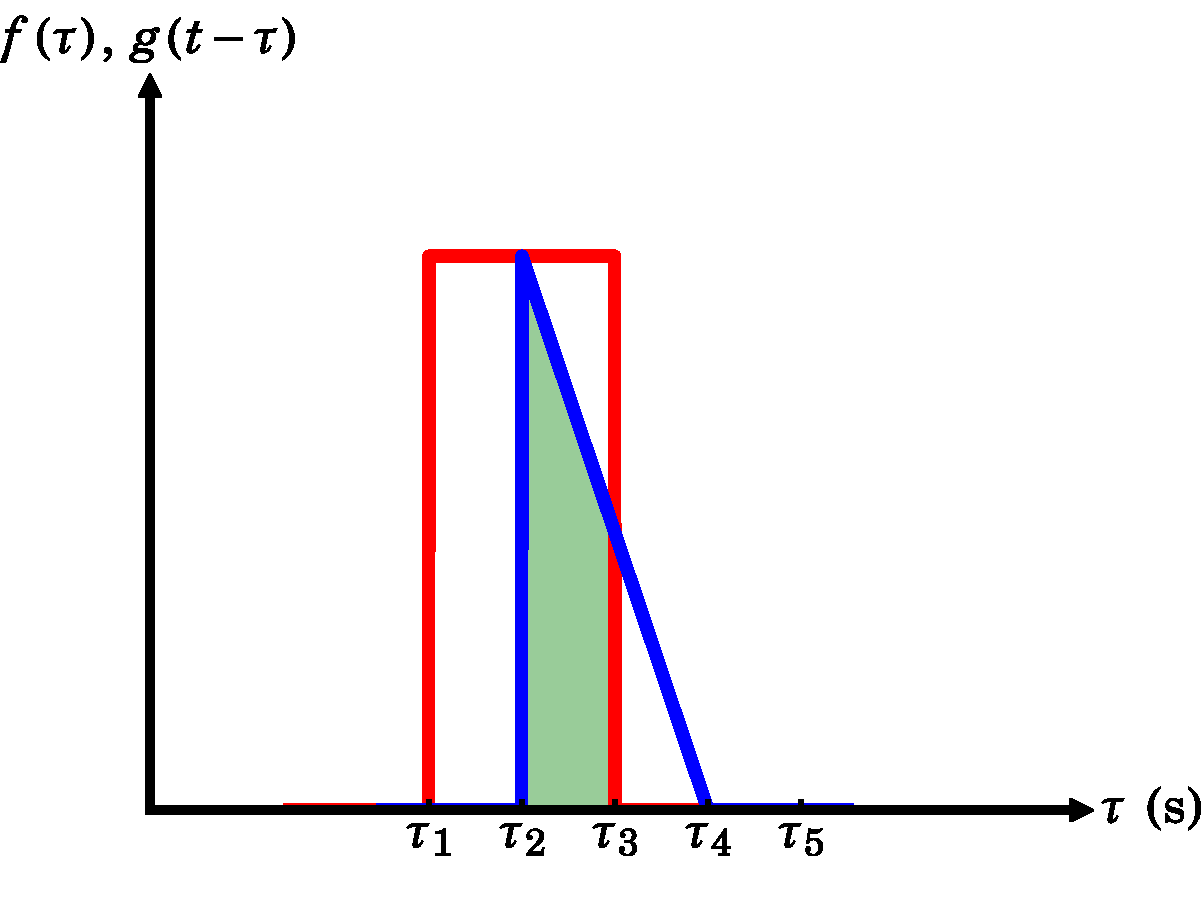
\includegraphics[width=0.32\textwidth]{figures/convolution_t4}
	\label{fig:conv_t4}
}
\subfloat[]{
	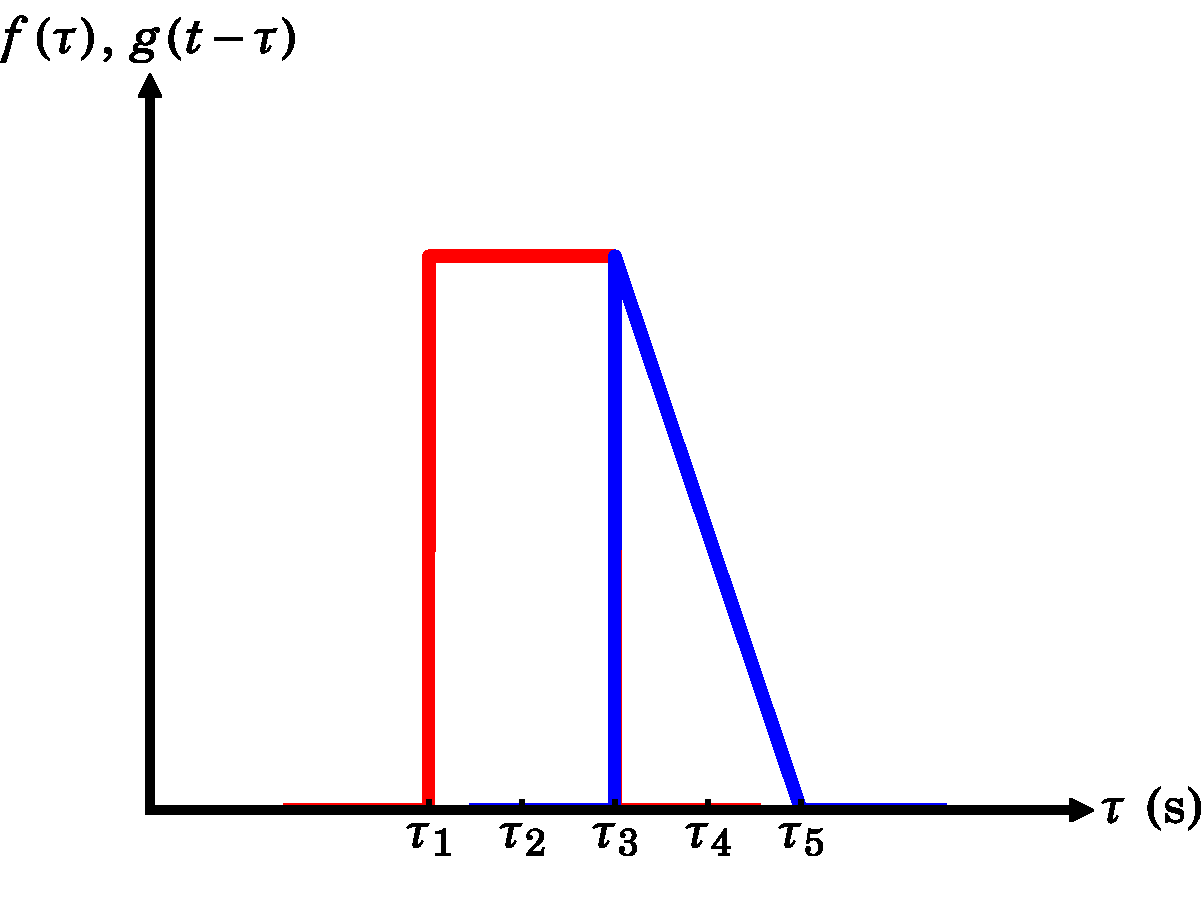
\includegraphics[width=0.32\textwidth]{figures/convolution_t5}
	\label{fig:conv_t5}
}
\subfloat[]{
	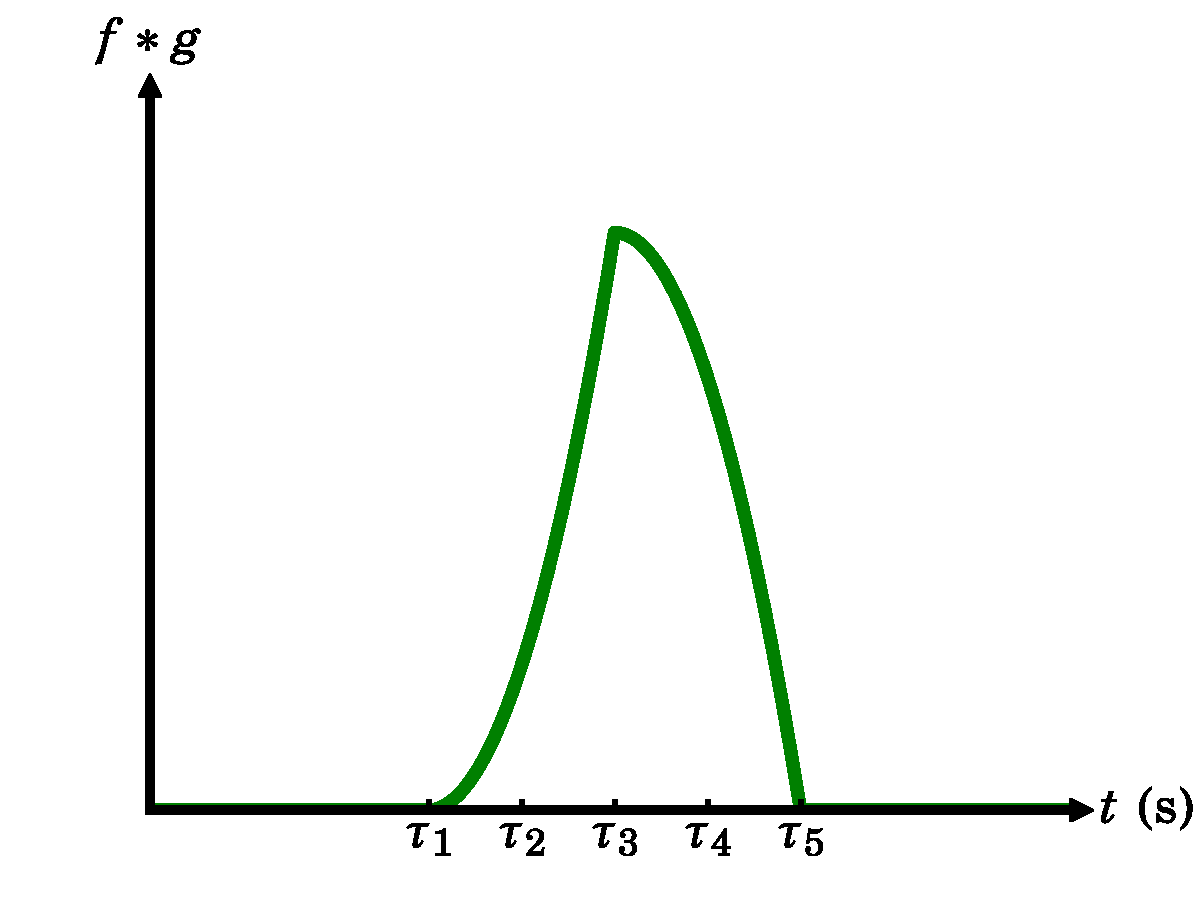
\includegraphics[width=0.32\textwidth]{figures/convolution_fgconv}
	\label{fig:conv_fgconv}
}
\caption[Graphical representation of convolution in the time domain.]{RERUN THESE AND CORRECT NON-ITALIC `t' IN AXIS!!!!!! Graphical representation of convolution in the time domain. Two functions $f\left(t\right)$ and $g\left(t\right)$, are shown in parts (a) and (b) respectively. To find the convolution of the two functions, one function is reversed in time--this is shown in part (c) (in this case $g\left(t\right)$ was chosen), and it is then translated across the other function, shown in parts (d) through to (h). The value of the convolution at any time, $\tau$, is the area overlap (shown as the highlighted areas in parts (d) through to (h)) of the two functions, when the leading non-zero value of the translated function is at $\tau$. The convolution function is shown in part (i).}\label{fig:convolution_time}
\end{center}
\end{figure}

Convolution can be thought of, much more simply, in the frequency domain. As explained by \citet[chap. 2]{Bracewell2000}, Convolution Theory states that the Fourier Transform of the convolution of two functions is the multiplication of the Fourier transforms of the functions. This can be written as:
\begin{align}
\mathcal{F}\left\{f \ast g\right\} = \mathcal{F}\left\{f\right\} \cdot \mathcal{F}\left\{g\right\} \label{eqn:convolutionTheoryFDom}
\end{align}
where $\mathrm{\mathcal{F}}$ is the Fourier transform function, and $f$ and $g$ are functions\footnote{The scalar product symbol ($\cdot$) is used in Equation~\ref{eqn:convolutionTheoryFDom} to avoid confusion with the vector product ($\times$), since the two Fourier transforms are multiplied on a point-by-point basis.}. The convolution of two functions in the frequency domain is illustrated in Figure~\ref{fig:convolution_freq}.
\begin{figure}[t]
\begin{center}
\subfloat[]{
	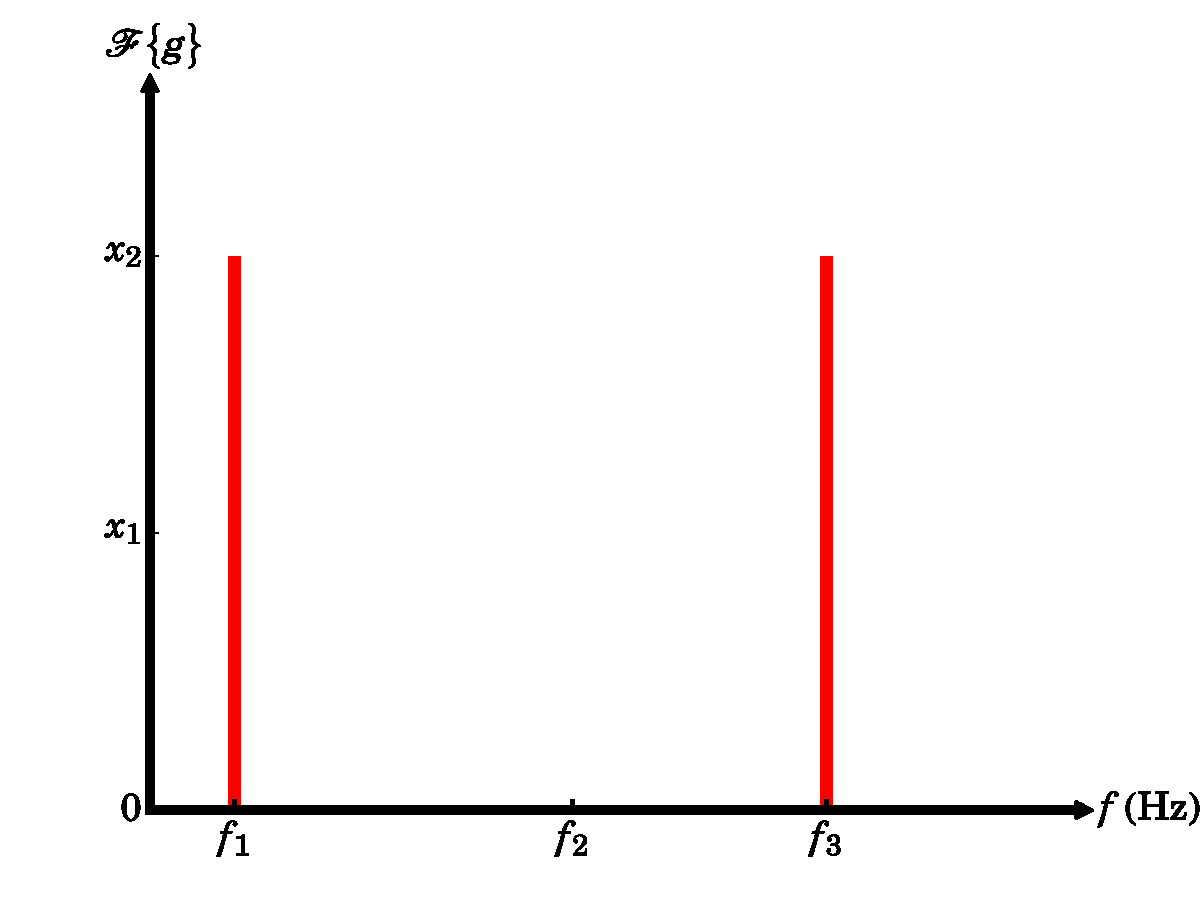
\includegraphics[width=0.48\textwidth]{figures/convolutionFdom_g}
	\label{fig:convFdom_g}
}
\subfloat[]{
	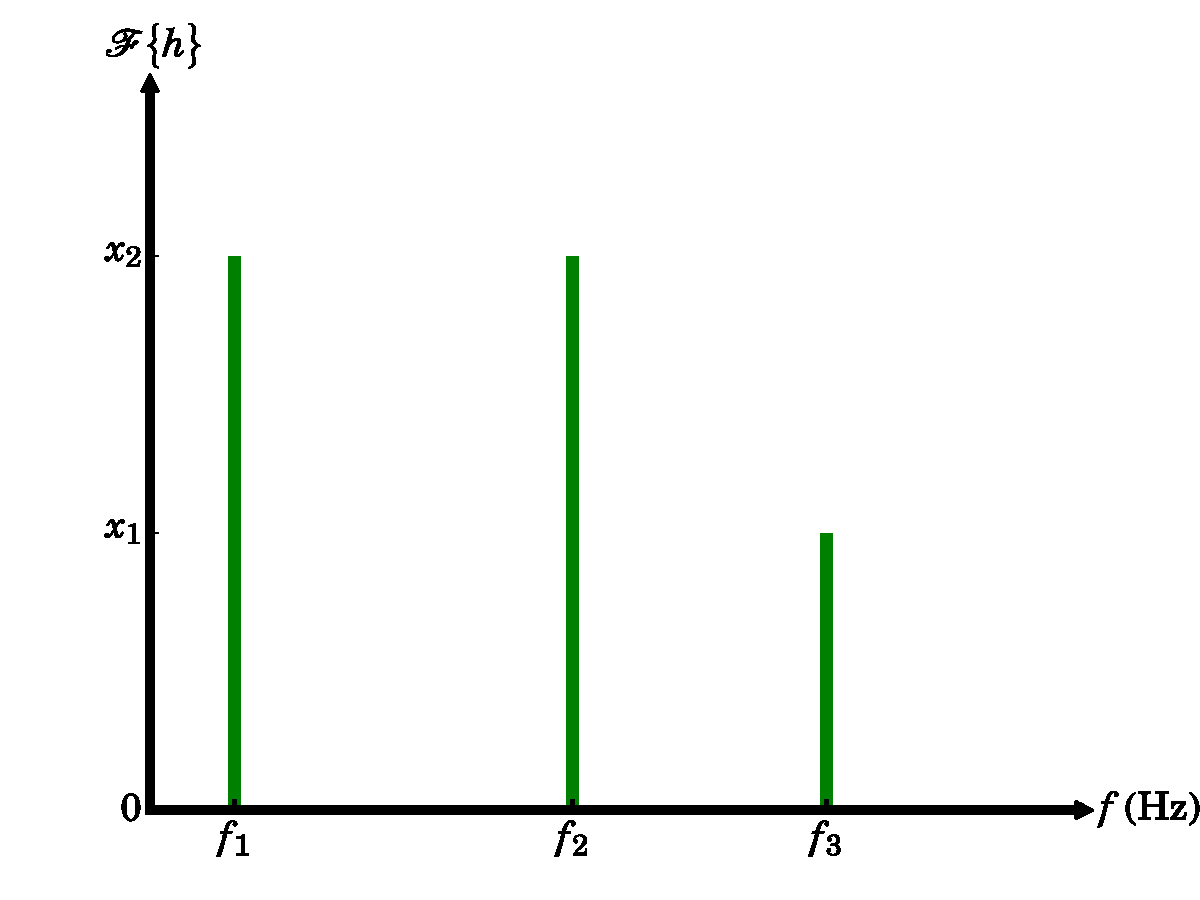
\includegraphics[width=0.48\textwidth]{figures/convolutionFdom_h}
	\label{fig:convFdom_h}
}
\\
\subfloat[]{
	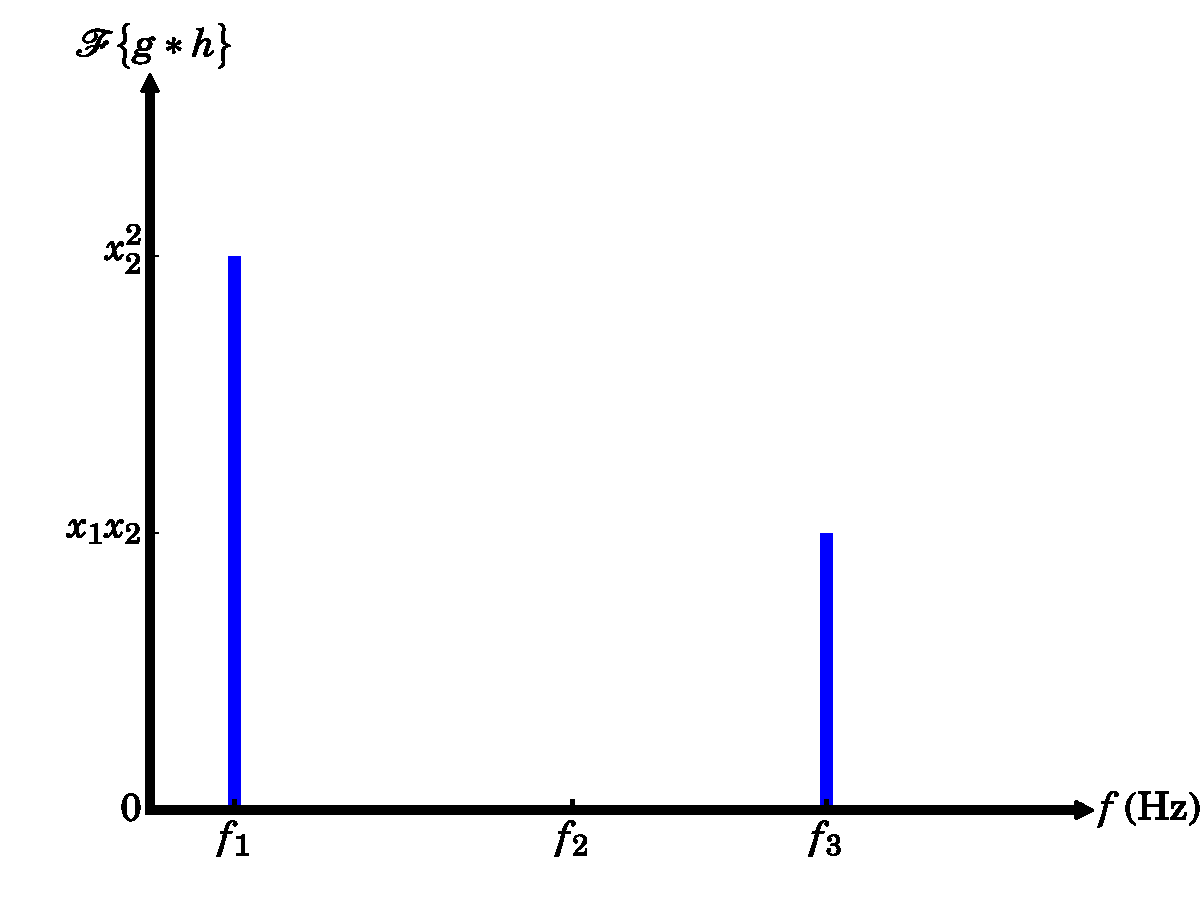
\includegraphics[width=0.48\textwidth]{figures/convolutionFdom_ghconv}
	\label{fig:convFdom_gh}
}
\caption[Convolution in the frequency domain.]{Convolution in the frequency domain. Two functions $g$ and $h$, whose Fourier transforms ($\mathcal{F}\left\{g\right\}$ and $\mathcal{F}\left\{h\right\}$) are shown in (a) and (b) respectively. (c) shows the Fourier transform of the convolution of $g$ and $h$ ($\mathcal{F}\left\{g \ast h\right\}$); it can be clearly seen that this is the same as the point-by-point multiplication of the two Fourier transforms of $g$ and $h$ (as is expected from the convolution theory).}
\label{fig:convolution_freq}
\end{center}
\end{figure}
%
\subsection{Cross Correlation}\label{ssec:crossCol}
Cross correlation is a mathematical process which can be used to measure the similarity of two functions or signals and is closely related to convolution. Mathematically, the cross correlation of two functions, $f\left(t\right)$ and $g\left(t\right)$, is defined as:
\begin{align}
\left(f \star g\right)\left(t\right) \stackrel{\mathrm{def}}{=}
\int_{-\infty}^{\infty} f^{\ast}\left(-\tau\right)g\left(t-\tau\right)\,\d\tau
	\,, \label{def:cross-correlation}
\end{align}
where $f^{\ast}$ is the complex conjugate of $f$. A quick comparison to the definition of the convolution (Equation~\ref{def:convolution}):
\begin{align}
\left(f \ast g\right)\left(t\right) \stackrel{\mathrm{def}}{=}  \int_{-\infty}^{\infty} f\left(\tau \right)g\left(t - \tau \right)\,\d\tau \,,
\tag{Equation~\ref{def:convolution} revisited}
\end{align}
shows that the convolution and cross correlation are simply related by:
\begin{align}
f\left(t\right) \star g\left(t\right) = 
	f^{\ast}\left(-t\right) \ast g\left(t\right) \,.
\end{align}
%
\subsection{Application of Cross Correlation to Detector Readout}
\label{ssec:appCrossCol}
In order to completely characterise a detector, it is important to measure the electronic noise generated within the detector itself; this is because it is this noise that will define the ultimate sensitivity of the detector (for a \gls{acr:CEB}-type detector the various internal noise sources have been covered in Section~\ref{sec:theory-noise}). The measurement of a detector's noise is complicated however, by the fact that the amplitude of internal noise in the detector is, in most cases, much less than the input-referred noise of the readout amplifier. While it is possibly to simply state that in any realistic scenario, the performance of the detector (in terms of sensitivity, at least) will be limited by the amplifier and thus it is justifiable to calculate the sensitivity of the detector based upon the noise of the readout amplifier; in a study of the detector itself (rather than an instrument utilising the detector), it is important to characterise the detector as completely as possible. This was one of the main reason for the switch from the readout amplifier described in Section~\ref{sec:initial_readout_system} to that described in Section~\ref{sec:Final_Readout}.
\par
Unfortunately, the INA103 based amplifier (described in Section~\ref{sec:Final_Readout}, which had an input-referred noise amplitude of $\sim 1~\mathrm{nV\,Hz}^{\nicefrac{1}{2}}$) was unable to directly measure the internal noise of the \gls{acr:CEB} detectors being studied. To address this, a novel readout and data-processing system was devised utilising two parallel \gls{acr:JFET}-buffered INA103 amplifiers (as shown in Figure~\ref{fig:finalAmp}) and cross correlating their outputs. The concept behind the design of this readout system was that, while the average noise amplitude of the two amplifiers would be the same, their noise spectra are not correlated, hence the cross-correlation techniques described above should be capable of removing the noise signal generated by the amplifier.\footnote{Since the exact amplitude and frequency spectrum of the amplifier noise is random, it is clear that multiple cross-correlated acquisitions may need to be combined to remove the amplifier noise.} On the other hand, the signal supplied to both amplifiers will be present and correlated in the output of both amplifiers and thus would be present after the two signals were cross correlated. The voltage output of the detector was split between the two amplifiers, with the output of each amplifier fed into a separate channel of a data acquisition system. Once the signals had been digitised by the data acquisition system, the two signals were cross correlated by National Instruments LabView software. A simplified process flow for the measurement of detector noise using this technique is shown in Figure~\ref{fig:crossCol_flow}.
\begin{figure}[tb]
\begin{center}
\includegraphics[width = 0.95\textwidth]{figures/crossCol_flow}
\caption[Cross-correlated noise measurement process flow]{Simplified process flow for measurement of low levels of electrical noise by utilising cross correlation of two signals from a common source. Intersections with dashed lines correspond to the example noise power spectra shown in Figure~\ref{fig:crossColNoiseEx}.}
\label{fig:crossCol_flow}
\end{center}
\end{figure}
\par
\begin{figure}[p]
\begin{center}
\subfloat[]{
	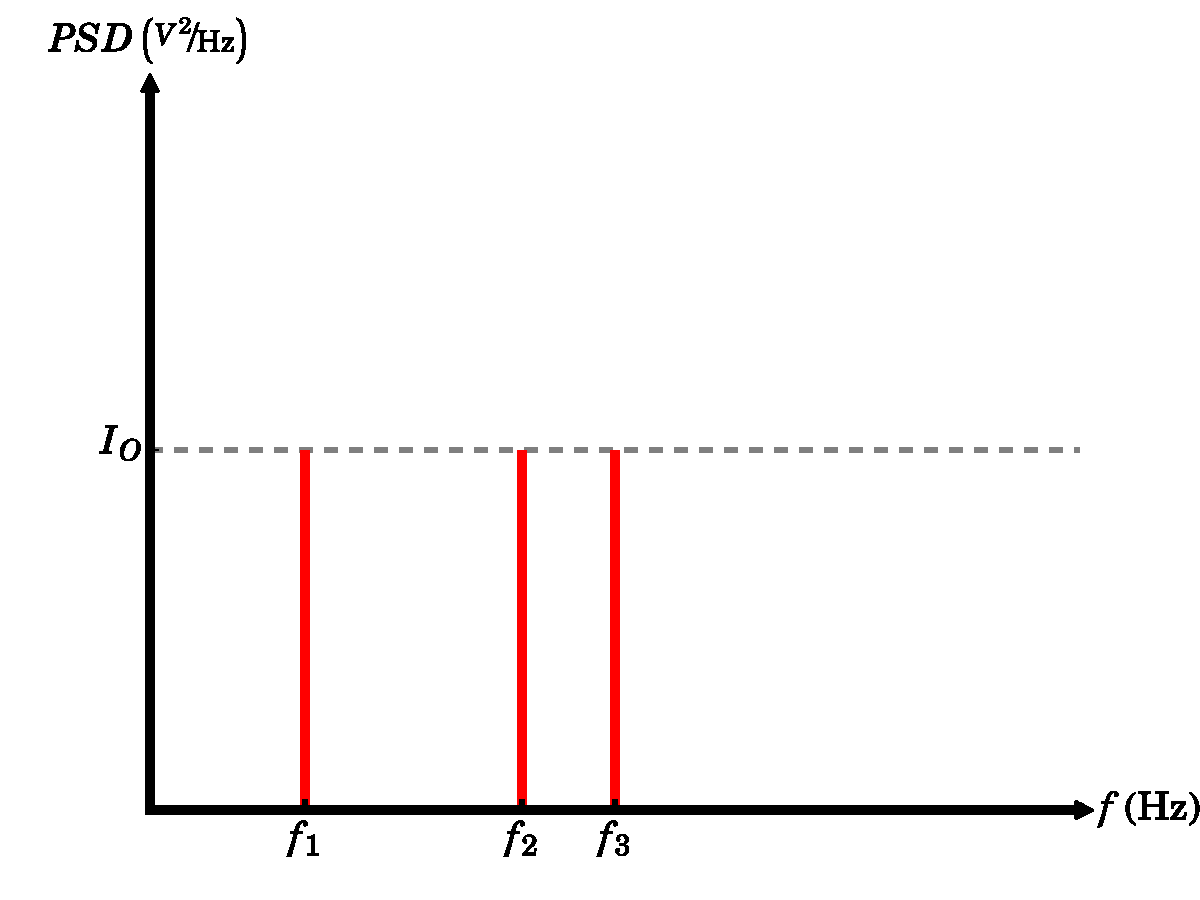
\includegraphics[width=0.48\textwidth]{figures/crossColNoiseEx_input}
	\label{fig:crossColNoiseEx_input}
}
\subfloat[]{
	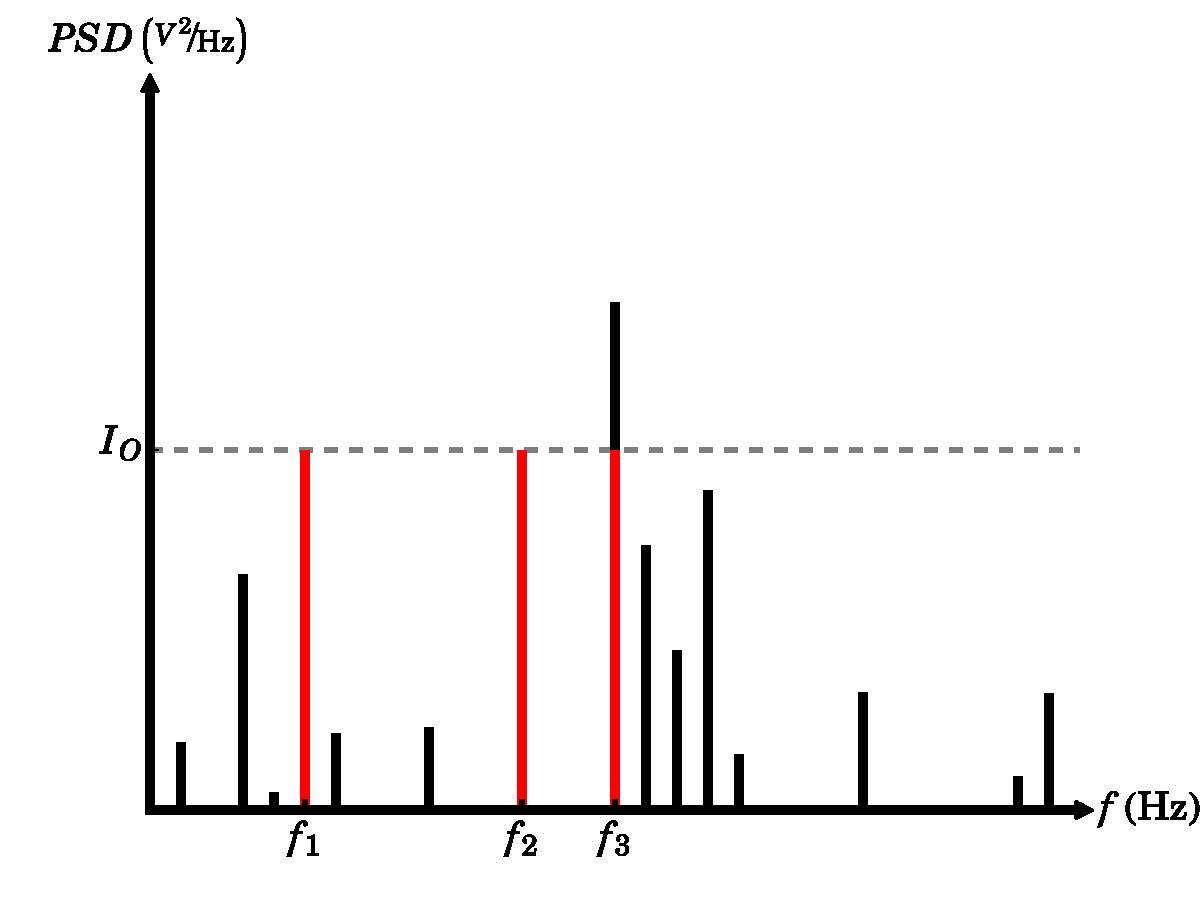
\includegraphics[width=0.48\textwidth]{figures/crossColNoiseEx_amp1}
	\label{fig:crossColNoiseEx_amp1}
}
\\
\subfloat[]{
	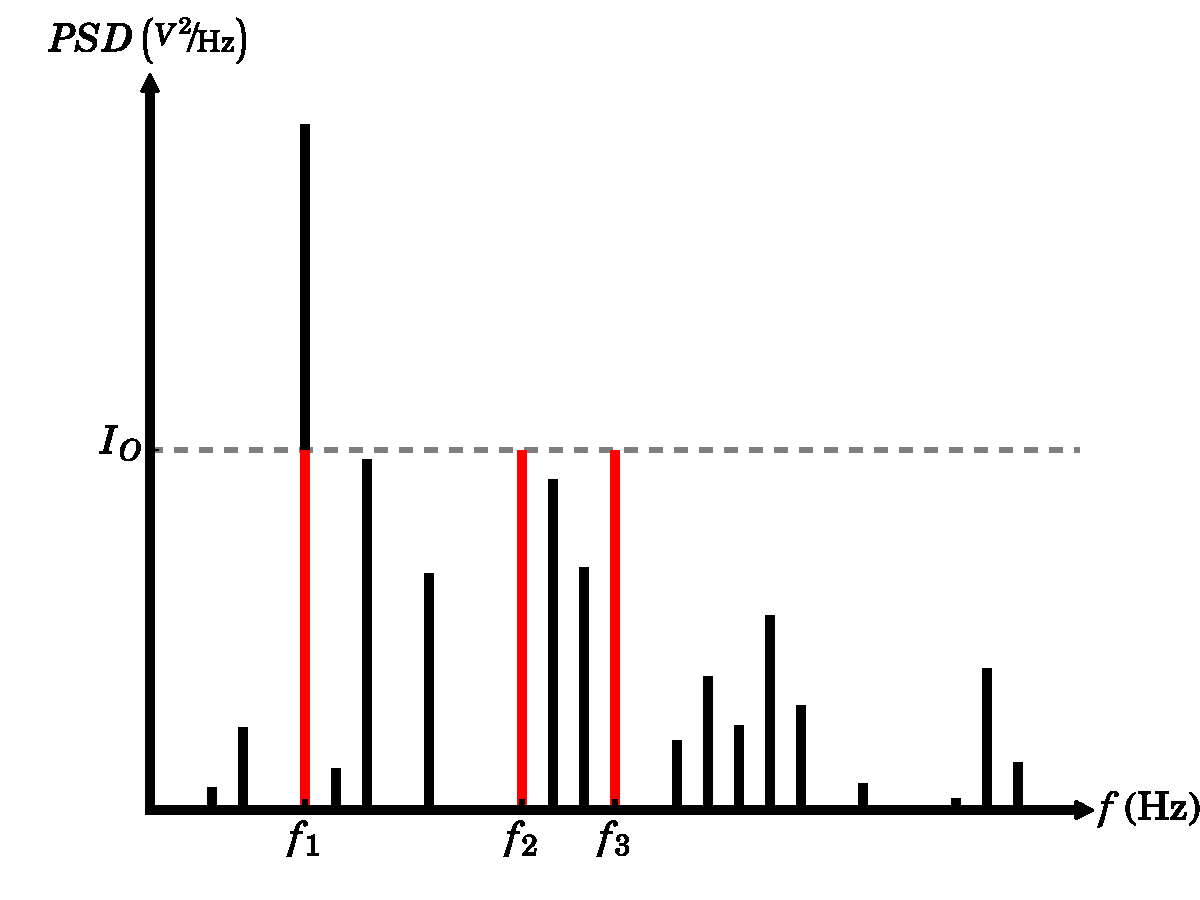
\includegraphics[width=0.48\textwidth]{figures/crossColNoiseEx_amp2}
	\label{fig:crossColNoiseEx_amp2}
}
\subfloat[]{
	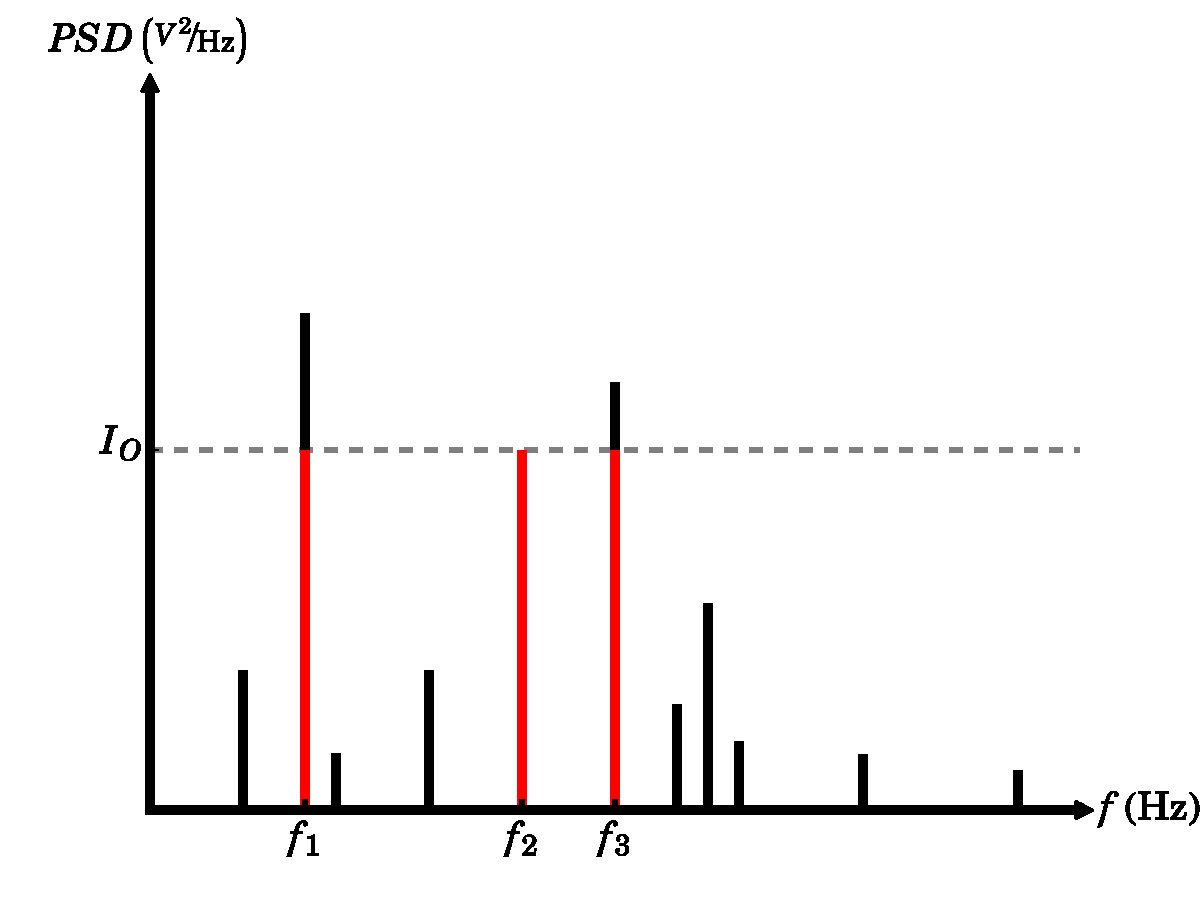
\includegraphics[width=0.48\textwidth]{figures/crossColNoiseEx_output}
	\label{fig:crossColNoiseEx_output}
}
\caption[Removal of amplifier noise from a measurement by the use of cross correlation.]{Removal of amplifier noise from a measurement by the use of cross correlation. (a) Power spectrum of detector output; the signal consists of three tones, each of intensity $I_{\mathrm{O}}$, at frequencies $f_{1}$, $f_{2}$ and $f_{3}$. (b) and (c) Outputs of the two parallel amplifiers; the signal (shown in red) is still present however the power spectra now also includes several other features including noise which has affected the signal at $f_{3}$ in (b) and $f_{1}$ in (c). (d) Output from readout system without any averaging; the majority of the noise introduced by the amplifiers has been removed (some features remain due to the random nature of the noise generated by the amplifiers, meaning that it is possible for features to exist at the same frequency in the outputs of both amplifiers, such features will \textit{survive} the cross correlation). The alteration to the signal at $f_{1}$ and $f_{3}$ has also been reduced. Subfigure numbering corresponds to the points at which the signal intersects with the dashed lines in Figure~\ref{fig:crossCol_flow}. (Colours for reference only.)}
\label{fig:crossColNoiseEx}
\end{center}
\end{figure} 
The effect of using cross correlation to remove electrical noise introduced by readout amplifiers is illustrated in Figure~\ref{fig:crossColNoiseEx}, which shows simplified examples of the noise power spectrum at various stages of the process flow shown in Figure~\ref{fig:crossCol_flow}---the spectra shown in Figure~\ref{fig:crossColNoiseEx} correspond to the points at which the process flow intercepts the dashed lines in Figure~\ref{fig:crossCol_flow}. Figure~\ref{fig:crossCol_flow} shows that, while the majority of the noise contributed by the amplifiers is successfully removed, some features remain; this is due to the random probability of both amplifiers generating a tone at a given frequency. When both noise spectra contain features at corresponding frequencies, there will also be a tone at the same frequency in the cross-correlated spectrum. While this cannot be avoided, the amplitude of these tones can be substantially reduced with averaging.
\par 
\begin{figure}[tb]
\begin{center}
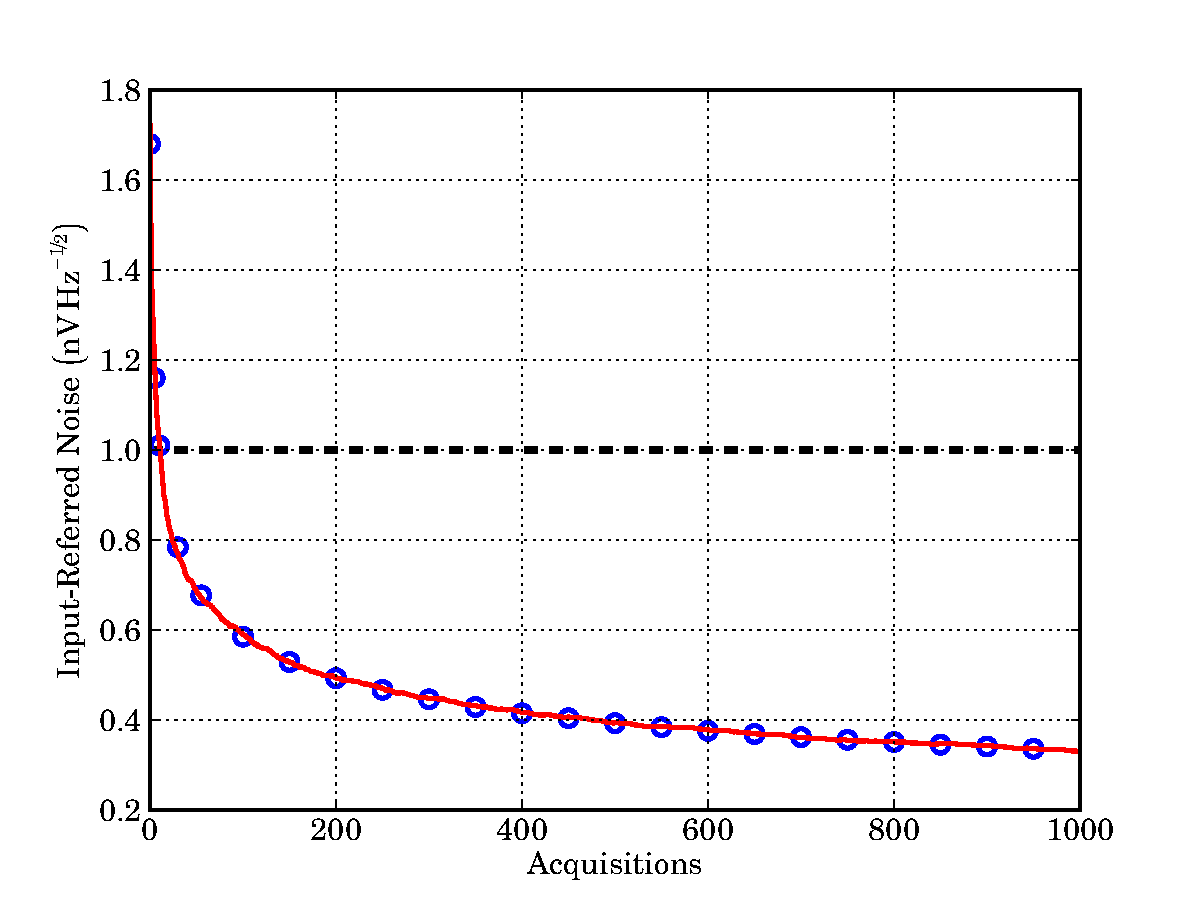
\includegraphics[width = 0.95\textwidth]{figures/crossColNoiseSimData}
\caption[Reduction in input-referred noise with increased number of averaged acquisitions for cross-correlated amplifiers]{Reduction in input-referred noise with increased number of averaged acquisitions for cross-correlated amplifiers. Solid line---simulation performed in National Instruments LabView software. Open circles---Experimental data. Dashed line---Expected input-referred noise for a single INA103 amplifier. It is clear that the simulation and experiemental data are in excellent agreement.}
\label{fig:crossCol_NoiseSimData}
\end{center}
\end{figure}
The performance of this readout system has been both simulated (using artificial signals generated by National Instruments LabView software) and measured experimentally. Both the simulation and the measurements were of the amplifiers having a shared connection to a short (equivalent to the scenario for measuring the input-referred noise of an amplifier used throughout the work covered in this chapter). Figure~\ref{fig:crossCol_NoiseSimData} shows the results of the simulation (solid line), along with experimental data (open circles)\footnote{For clarity, the experimental data have been reduced prior to plotting.} and the expected noise level resulting from one of the amplifiers operating singularly. It can be seen from Figure~\ref{fig:crossCol_NoiseSimData} that the simulation and measured data are in excellent agreement. Both the simulation and the measured data start above the specified amplifier noise; this is due to the mechanics of the noise measurement and the possibility of a single cross-correlated acquisition causing an increase in the noise. After a small number of acquisitions (approximately ten), the measured noise level has dropped to that of the input-referred noise of a single amplifier. With continued acquisitions, the noise level continues to drop until a constant level, well below the amplifiers' input-referred noise, is reached. This \textit{noise floor} is caused by the binning of the waveform in the sampling process and the random probability of a noise feature at each of the binned frequencies in the Fourier transform of the sampled data. The minimum achieved input-referred noise of the cross-correlated amplifier setup was found to be approximately $330~\mathrm{pV\,Hz}^{\nicefrac{-1}{2}}$.
%
\section{Summary of Readout and Biasing Systems}
As has been covered in this chapter, a number of systems have been developed and used to measure \gls{acr:SiCEB} detectors. While the majority of the measurements presented in this work were performed with the equipment described in Section~\ref{sec:Final_Readout} (with succesful measurements of the device and photon noise performed using the techniques described in Section~\ref{sec:cross_col_noise}), some early measurements were performed with the systems described earlier in this chapter (where this is the case, it has been made apparent). A summary of the performance of the various bias systems and readout amplifiers described throughout this chapter is given in Tables~\ref{tab:biasSystems} and \ref{tab:readoutSystems} respectively.

\begin{table}[htb]
\caption[Summary of detector bias systems]{Summary of detector bias systems.} 
\label{tab:biasSystems}
\centering
\begin{threeparttable}
\begin{tabular*}{0.8\textwidth}{lS[table-format=1.2]l}
\toprule\toprule
{System} & {Bias Jitter $\left(\mathrm{\upmu A}\right)$} & {Notes} \\
\midrule
Keithley 220 & 0.55 & See below\tnote{a} \\
Initial custom bias generator\tnote{b} & 1.00 & \\
Final custom bias generator\tnote{c} & 0.80 & \\
\bottomrule
\end{tabular*}
\begin{tablenotes}
\item[a] This unit caused substantial levels of electrical noise to be introduced into the measurement (as seen in Figure~\ref{fig:Keithley220_noise}).
\item[b] Based upon Analog Devices' AMP03 amplifier.
\item[c] Based upon Analog Devices' OP470 amplifier.
\end{tablenotes}
\end{threeparttable}
\end{table}

\begin{table}[htb]
\caption[Summary of detector readout systems]{Summary of detector readout systems.} 
\label{tab:readoutSystems}
\centering
\begin{tabular*}{\textwidth}{lS[table-format=4.0]c
						S[table-format=3.0]S[table-format=2.2]}
\toprule\toprule
{System}&{Gain}&{Input Range $\left(\mathrm{mV}\right)$}&{$3\mbox{-}\mathrm{dB}$ BW $\left(\mathrm{kHz}\right)$}&{IRN $\left(\mathrm{nV\,Hz}^{\nicefrac{-1}{2}}\right)$} \\[1.1pt] \midrule
Initial System & 1000 & $\pm 12.7$ & 55 & 10.00\\[1.1pt]
Final System & 600 & $^{+29.3}_{-\hphantom{2} 7.3}$ & 240 & 0.85 \\[1.1pt]
\parbox[t]{\widthof{Cross-Correlation}}{Final System w/ \\ Cross-Correlation} & 600 & $^{+29.3}_{-\hphantom{2} 7.3}$ & 240 & 0.33 \\[1.1pt]
\bottomrule
\end{tabular*}
\end{table}

% ********** End of chapter **********
